% siminos/talks/GTmath12/sectSlice.tex      pdflatex sectSlice
% $Author: predrag $
% $Date: 2012-02-14 14:32:06 -0500 (Tue, 14 Feb 2012) $

% remember to always update
%	dasbuch/WWW/overheads/continuous/continuous.pdf

% Predrag GT math colloquium                2012.03.26
% derived from
% talks/predrag/continuous/continuous.tex   2011.09.09
% Predrag beamer format                     2011.06.17
% Predrag                                   2011.04.12
% derived from
% siminos/talks/Dresden10/symmReduc.tex 	2010.06.29
% Predrag Eckmann's haeberli slide style    2005.05.03
%    ChaosBook/version 11 slides
%	 from ChaosBook continuous.tex

% might want to use text from
%    predrag/lectures/Goth11/Cphg11abstr.txt
%    predrag/lectures/maribor/11/abscvitancourse.tex

\input ../../inputs/layoutBeamer
\input ../../inputs/def % no edits, always from dasbuch/book/inputs
\input ../../inputs/defsBeamer
                          \date{\textcolor{yellow}{\scriptsize
 16 March 2012
                          }}

\title{{\Huge got symmetry?}
       \\
       {here is how you slice it}}
%\author{Predrag Cvitanovi\'c}
\author[Cvitanovi\'c]
{
  \textcolor{green!50!black}{
  {Predrag~Cvitanovi\'c}
  }
}
\institute
{
%  \inst{1}%
CDSNS Colloquium \\
School of Mathematics, Georgia Tech
}

\begin{document}

\begin{frame}
  \titlepage
\end{frame}

%\begin{frame}{Outline}
%  \tableofcontents
%\end{frame}

\section[dynamical systems]{dynamical systems}

\subsection[dynamical systems]{dynamical systems}

\begin{frame}{dynamical description of turbulent flows}
%	from {../chapter/dynsysII}

\begin{block}{\statesp}
a manifold $\pS \in \reals^{d}$ :
$d$ numbers determine the state of the system
\end{block}

\bigskip

\begin{block}{representative point }
$\ssp(t) \in \pS$
\\
a state of physical system at instant in time
\end{block}
\end{frame}

\begin{frame}{today's experiments}
\begin{block}{example of a representative point }
$\ssp(t) \in \pS$, $d= \infty$ \\
a state of turbulent pipe flow at instant in time
\end{block}

\bigskip

%%%%%%%%%%%%%%%%%%%%%%%%%%%%%%%%%%%%%%%%%%%%%%%%%%%%%%%%%%%%%%%%%%
%\hfill
%\begin{minipage}[c]{0.35\textwidth}
Stereoscopic Particle Image Velocimetry $\to$
3-$d$ velocity field over the entire pipe%
\footnote{
%"Stereoscopic PIV on transition in pipe flow",
Casimir W.H. van Doorne
(PhD thesis, Delft  2004)
%; 	{\tt www.ahd.tudelft.nl}
}

\bigskip

\begin{center}
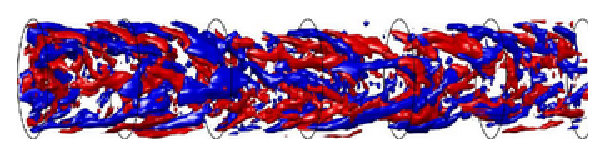
\includegraphics[width=0.90\textwidth]{vDoorne4}
\end{center}
\end{frame}

\begin{frame}{}
\begin{block}{deterministic dynamics}
map $\timeflow(\xInit)$ =
representative point time $t$ later
\end{block}

\begin{block}{evolution}
\begin{center}
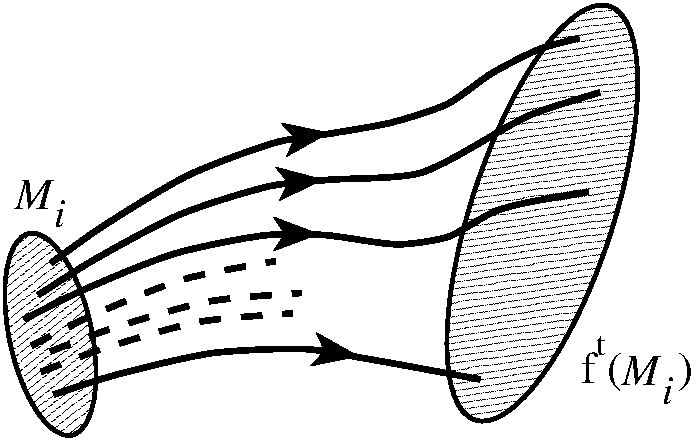
\includegraphics[width=0.40\textwidth]{f_flow}
\end{center}
$\timeflow$ maps a region $\pS_i$ of
the {\statesp} into the region $\flow{t}{\pS_i}$.
\end{block}
\end{frame}

\begin{frame}{have : chart over 61,506 dimensional \statesp\ of turbulent flow}
\begin{center}
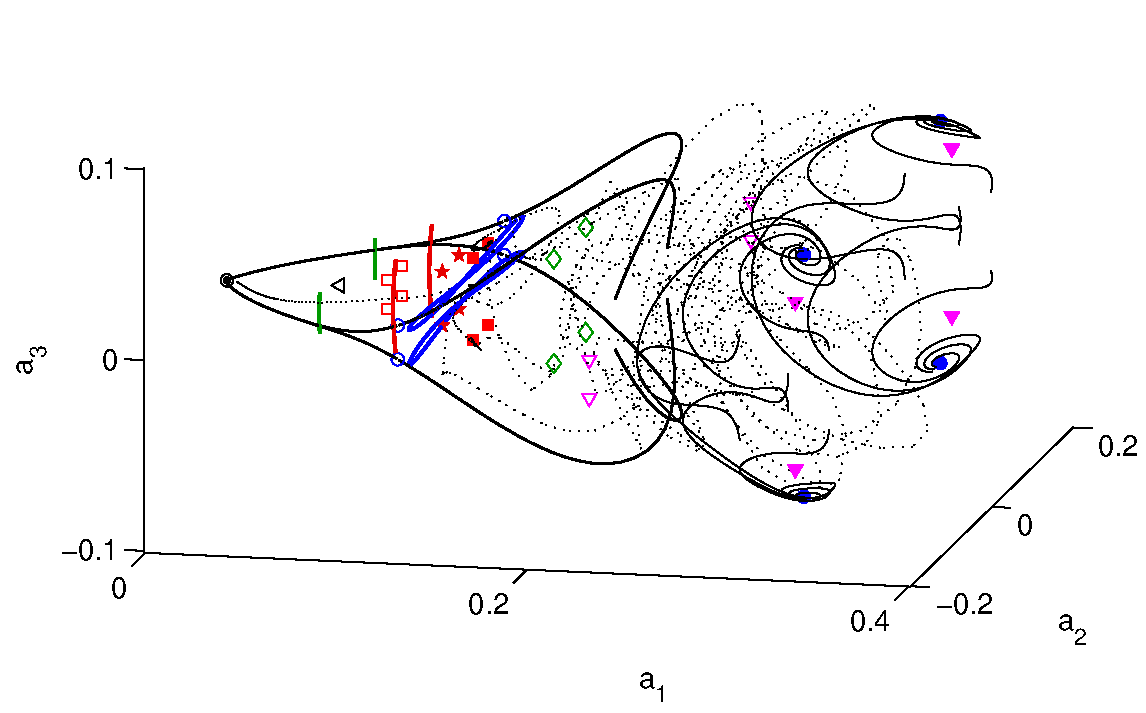
\includegraphics[width=0.80\textwidth]{statespace_123}
\end{center}
\eqva\ of turbulent plane Couette flow,
their unstable manifolds, and a turbulent video mapped out as one happy family

\bigskip

\hfill   {\small
          for movies, please click through
            \textcolor{blue}{\href{http://ChaosBook.org/tutorials}
             {ChaosBook.org/tutorials}}
          }
\end{frame}

%%%%%%%%%%%%%%%%%%%%%%%%%%%%%%%%%%%%%%%%%%%%%%%%%%%%%%%%%%%%%%%%%%%%%%%%%%%%
\section[Das Problem]{the problem with symmetry}


\begin{frame}{}
today's talk's focus:
\begin{block}{}
{\Huge
nature loves symmetry
}
\end{block}
\end{frame}

\begin{frame}{symmetry of a dynamical system}
\begin{block}{a group $\Group$ is a {symmetry} of the dynamics if}
for every solution $f(\ssp) \in \pS$ and  $\LieEl \in \Group$,
$\LieEl f(\ssp)$ is also a solution
\end{block}
\end{frame}


\begin{frame}{example: $\SOn{2}_z\times \On{2}_\theta$ symmetry of pipe flow}
            \begin{block}{}
 %% A27*-pipeSymms.* - read dasbuch/book/FigSrc/inkscape/00ReadMe.txt
 \begin{center}
  \setlength{\unitlength}{0.35\textwidth}
  %% \unitlength = units used in the Picture Environment
(a)
  \begin{picture}(1,0.52454249)%
    \put(0,0){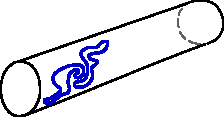
\includegraphics[width=\unitlength]{A27a-pipeSymms}}%
    \put(0.61583231,0.13683004){\color[rgb]{0,0,0}\makebox(0,0)[lb]{\smash{$z$}}}%
    \put(0.00611823,0.27217453){\color[rgb]{0,0,0}\makebox(0,0)[lb]{\smash{$\theta$}}}%
  \end{picture}%
(b)
  \begin{picture}(1,0.52454249)%
    \put(0,0){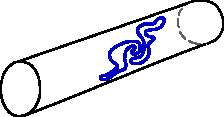
\includegraphics[width=\unitlength]{A27b-pipeSymms}}%
    \put(0.61583231,0.13683004){\color[rgb]{0,0,0}\makebox(0,0)[lb]{\smash{$z$}}}%
    \put(0.00611823,0.27217453){\color[rgb]{0,0,0}\makebox(0,0)[lb]{\smash{$\theta$}}}%
  \end{picture}%
\\
(c)
  \begin{picture}(1,0.52454249)%
    \put(0,0){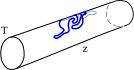
\includegraphics[width=\unitlength]{A27c-pipeSymms}}%
    \put(0.61583231,0.13683004){\color[rgb]{0,0,0}\makebox(0,0)[lb]{\smash{$z$}}}%
    \put(0.00611823,0.27217453){\color[rgb]{0,0,0}\makebox(0,0)[lb]{\smash{$\theta$}}}%
  \end{picture}%
(d)
  \begin{picture}(1,0.52454249)%
    \put(0,0){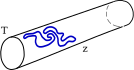
\includegraphics[width=\unitlength]{A27d-pipeSymms}}%
    \put(0.61583231,0.13683004){\color[rgb]{0,0,0}\makebox(0,0)[lb]{\smash{$z$}}}%
    \put(0.00611823,0.27217453){\color[rgb]{0,0,0}\makebox(0,0)[lb]{\smash{$\theta$}}}%
  \end{picture}%
 \end{center}
relative periodic solution: recurs at
time $\period{p}$, shifted by a streamwise translation, azimuthal rotation
$g_p$
			\end{block}
%	\end{columns}
% \caption{\label{fig:A27-pipeSymms}
			\begin{exampleblock}{}
\begin{itemize}
  \item[b)]  stream-wise recurrent
  \item[c)]  stream-wise, azimuthal recurrent
  \item[d)]  azimuthal flip recurrent
\end{itemize}
			\end{exampleblock}
\end{frame}


\subsection[{\cLf} example]{prelude: {\cLf} example}

\begin{frame}{\Large Das Problem}
\begin{block}{}
    {\large
% physicists
mathematicians like symmetry more than Nature
    }

\bigskip

\hfill
Rich Kerswell
\end{block}
\end{frame}

\begin{frame}{turbulence in pipe flows}
pipe flows : amazing data! amazing numerics!
\begin{center}
  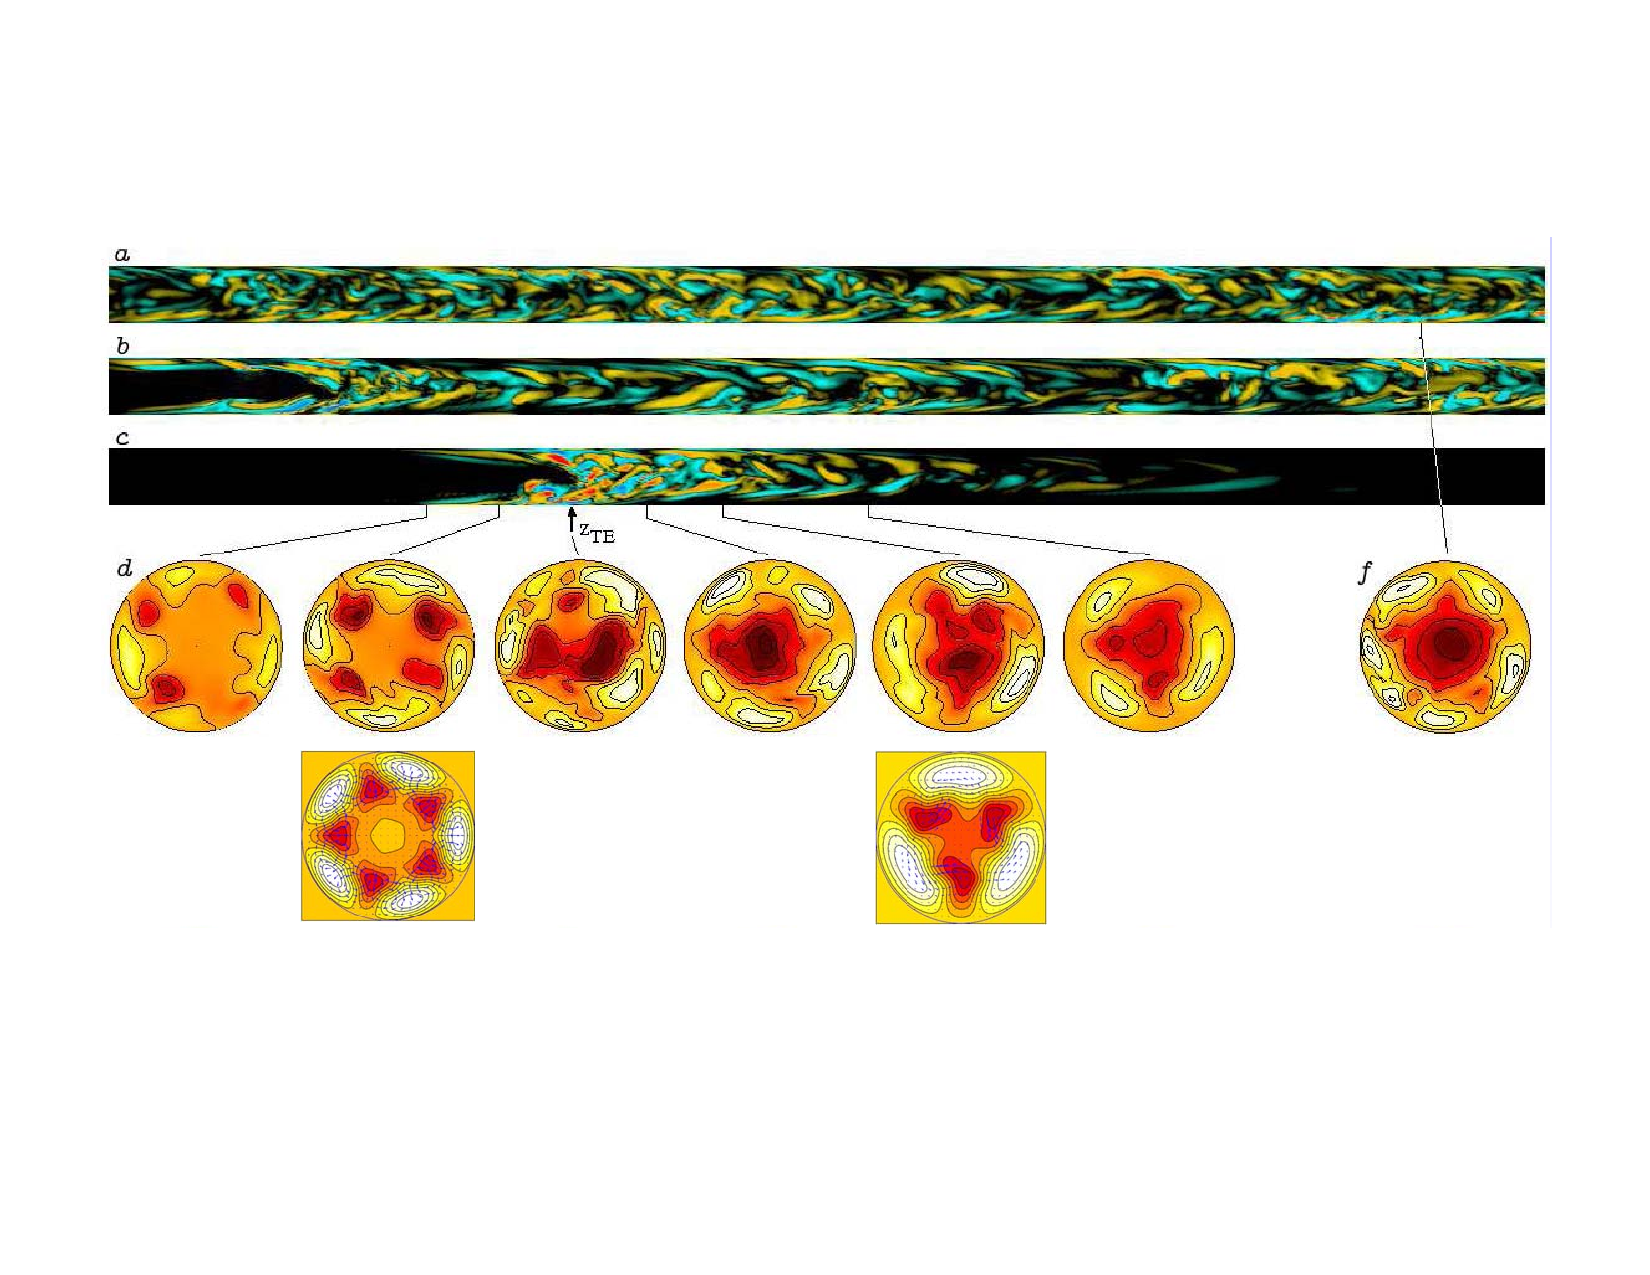
\includegraphics[width=1.0\textwidth,clip=true]
                    {pipeSects}
\end{center}

\bigskip
Nature, she don't care :
turbulence breaks all symmetries
\end{frame}

\begin{frame}{\Large Das Problem}
\begin{block}{drifting is energetically cheap}
flows are lazy, rather than doing work, solutions drift along non-shape-changing
symmetry directions
\end{block}
\end{frame}



\begin{frame}{\Large Das Problem}
% \begin{frame}{from {\cLf} $5D$ attractor $\to$ unimodal map}
	\begin{columns}[t]
	\column{.6\textwidth}
			\begin{exampleblock}{{\cLe}}
\scriptsize		
\[
		\left[
					\begin{array}{c}
				\dot{x}_1 \\ \dot{x}_2 \\ \dot{y}_1 \\ \dot{y}_2 \\ \dot{z}
				\end{array}
		\right]
=
		\left[
					\begin{array}{c}
				 -\sigma x_1 + \sigma y_1 \\
				-\sigma x_2 + \sigma y_2 \\
                (\RerCLor-z) x_1 - \ImrCLor x_2 -y_1-e y_2 \\
                \ImrCLor x_1 + (\RerCLor-z) x_2 + e y_1- y_2 \\
				-b z + x_1 y_1 + x_2 y_2
				\end{array}
		\right]
\]
$\RerCLor=28, \ImrCLor=0, b=8/3, \sigma=10, e= 1/10$
			\end{exampleblock}
            \begin{block}{}
  \begin{itemize}
  \item A typical $\{x_1,x_2,z\}$ trajectory
  \item superimposed:
  a trajectory  whose initial
  point is close to the \reqv\ $Q_{1}$
  \end{itemize}
            \end{block}
	\column{.40\textwidth}
 		\begin{exampleblock}{attractor}
        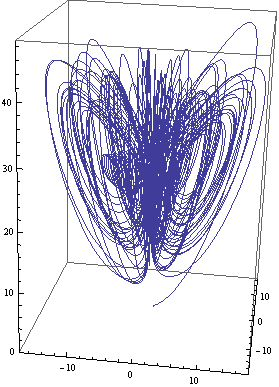
\includegraphics[width=\textwidth,clip=true]
                        {CLEx1x2z} %CLEx1x2zRelEqu}
		\end{exampleblock}
	\end{columns}
\end{frame}

\begin{frame}{} %{\statesp\ portrait of \cLf\ solutions}
\begin{block}{continuous symmetry induces drifts}
\begin{center}
  \includegraphics[width=0.35\textwidth,clip=true] %,height=0.5\textheight
  {CLEchaotic}
  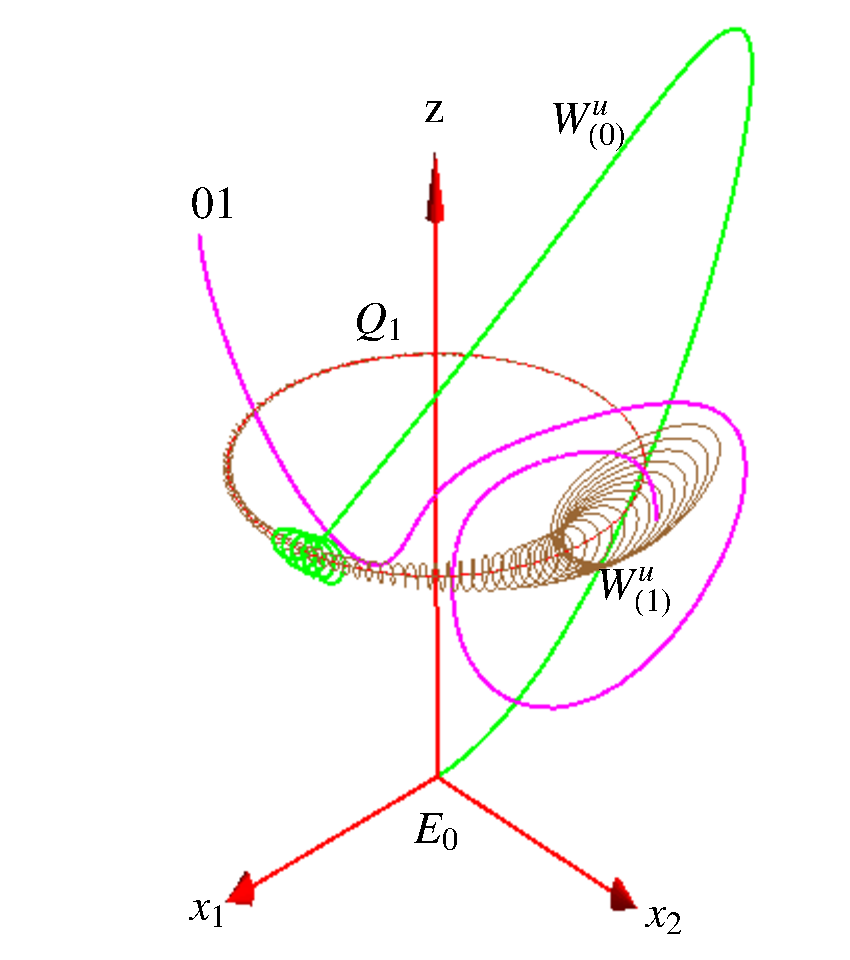
\includegraphics[width=0.35\textwidth,clip=true]
  {CLEcompact}
\end{center}
\end{block}
\begin{itemize}
  \item generic chaotic trajectory (blue)
  \item $E_0$ \eqv  %\EQV{0}
  \item $E_0$ unstable manifold - a cone of such (green)
  \item $Q_1$ \reqv\ (red)
  \item $Q_1$ unstable manifold, one for each point on $Q_1$ (brown)
  \item \rpo\ \cycle{01} (purple)
\end{itemize}
\end{frame}

\begin{frame}{
         \only<1>{
das Durcheinander
         }
         \only<2>{
\Large die L\"osung
        }
            }
% \begin{frame}{from {\cLf} $5D$ attractor $\to$ unimodal map}
	\begin{columns}[t]
	\column{.6\textwidth}
			\begin{block}{what to do?}
it's a mess
			\end{block}
			\begin{block}{the goal}
 reduce this messy strange attractor
to something simple
			\end{block}
	\column{.40\textwidth}
         \only<1>{
		\begin{exampleblock}{attractor}
        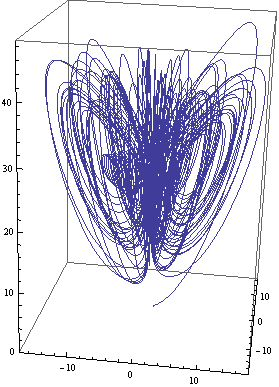
\includegraphics[width=\textwidth,clip=true]
                        {CLEx1x2z} %CLEx1x2zRelEqu}
		\end{exampleblock}
                }
         \only<2>{
		\begin{exampleblock}{symmetry \reducedsp}
  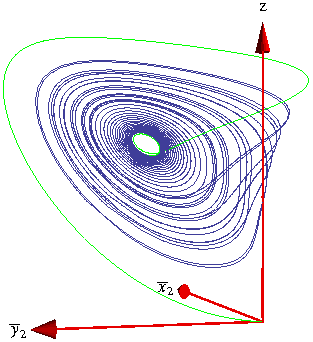
\includegraphics[width=\textwidth,clip=true]
  {CLEinvXYZ} %CLEip1}
		\end{exampleblock}
        \hfill  \textcolor{red}{amazing!}
                }
	\end{columns}
\end{frame}

\begin{frame}{\Large Das Gebot}
\begin{block}{}
    {\large
what I teach you now you must do
    }
\end{block}
\end{frame}

\section[relativity for cyclists]{relativity for cyclists}

\subsection[in/equivariance]{}

\begin{frame}{symmetries of dynamics}
  \begin{columns}
  \column{0.45\textwidth}
\begin{block}{time evolution}
%\label{fig:tangents}
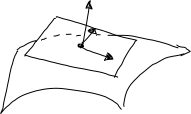
\includegraphics[width=0.90\textwidth]{A27groupTan}
\end{block}
  \column{0.55\textwidth}
$\vel(\ssp)$ : tangent along the time flow

\bigskip

$\groupTan^{(1)}(\ssp)$, $\groupTan^{(2)}(\ssp)$ : two group tangents
along infinitesimal symmetry shifts
	\end{columns}

\bigskip

\begin{block}{a flow $\dot{\ssp}= \vel(\ssp)$ is $\Group$-equivariant if}
\[
\vel(\ssp)=\LieEl^{-1} \, \vel(\LieEl \, \ssp)
\,,\qquad \mbox{for all } \LieEl \in {\Group}
\,.
\] %ee{eq:FiniteRot}

\end{block}

\bigskip

equations of motion of the same form in all frames
\end{frame}

\begin{frame}{example: \SOn{2} invariance}
			\begin{exampleblock}{{\cLe}}
\scriptsize		
\[
		\left[
					\begin{array}{c}
				\dot{x}_1 \\ \dot{x}_2 \\ \dot{y}_1 \\ \dot{y}_2 \\ \dot{z}
				\end{array}
		\right]
=
		\left[
					\begin{array}{c}
				 -\sigma x_1 + \sigma y_1 \\
				-\sigma x_2 + \sigma y_2 \\
                (\RerCLor-z) x_1 - \ImrCLor x_2 -y_1-e y_2 \\
                \ImrCLor x_1 + (\RerCLor-z) x_2 + e y_1- y_2 \\
				-b z + x_1 y_1 + x_2 y_2
				\end{array}
		\right]
\]
			\end{exampleblock}

\begin{block}{}
invariant under a \SOn{2} rotation by finite angle
\gSpace:
\scriptsize		
\[
\LieEl(\gSpace) \,=\,  \left(\barr{ccccc}
  \cos \gSpace  & \sin \gSpace  & 0 & 0 & 0 \\
 -\sin \gSpace  & \cos \gSpace  & 0 & 0 & 0 \\
 0 & 0 &  \cos \gSpace & \sin \gSpace   & 0 \\
 0 & 0 & -\sin \gSpace & \cos \gSpace   & 0 \\
 0 & 0 & 0             & 0              & 1
    \earr\right)
\] %{CLfRots}
\end{block}
%\begin{block}{\statesp\ decomposition}
%\begin{enumerate}
%  \item $m=0$ \SOn{2}-invariant subspace: $z$-axis
%  \item $m=1$ subspace with multiplicity 2
%\end{enumerate}
%\end{block}
\end{frame}

\begin{frame}{trajectories, orbits}
%  \caption{\label{fig:A27wurst}
	\begin{columns}[t]
	\column{.32\textwidth}
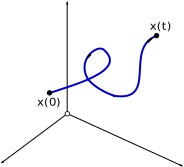
\includegraphics[width=0.95\textwidth]{A27traj}

trajectory $\ssp(\zeit)$
	\column{.32\textwidth}
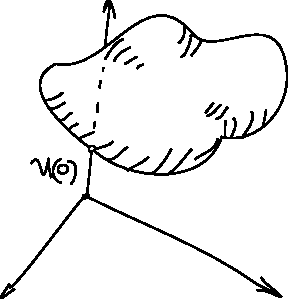
\includegraphics[width=0.95\textwidth]{A27gOrbit}

group orbit $\LieEl\,\ssp(0)$
	\column{.32\textwidth}
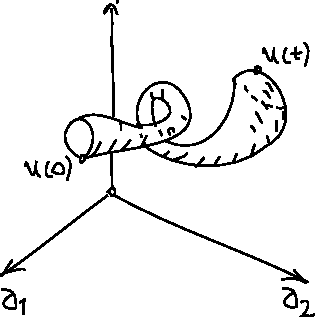
\includegraphics[width=0.95\textwidth]{A27wurst}

wurst $\LieEl\,\ssp(\zeit)$
	\end{columns}
\end{frame}

\begin{frame}{group orbits}
for any $\ssp \in \pS$, the
\textcolor{blue}{group orbit} $\pS_\ssp $ of $\ssp$ is the set of all group
actions
\[
\pS_\ssp = \{\LieEl\,\ssp \mid \LieEl \in {\Group}\} \subset \pS
\]

\bigskip\bigskip
states in $\pS_\ssp $ are physically equivalent
\end{frame}

\begin{frame}{stratification by group orbits}
  \begin{columns}
  \column{0.5\textwidth}
\begin{block}{group orbits}
% 2011-08-23 Predrag: previously BeThTraj.pdf from
% dasbuch/book/FigSrc/inkscape/BeThTraj.svg
%  2011-09-09 Predrag: updated continuous.tex overheads
%  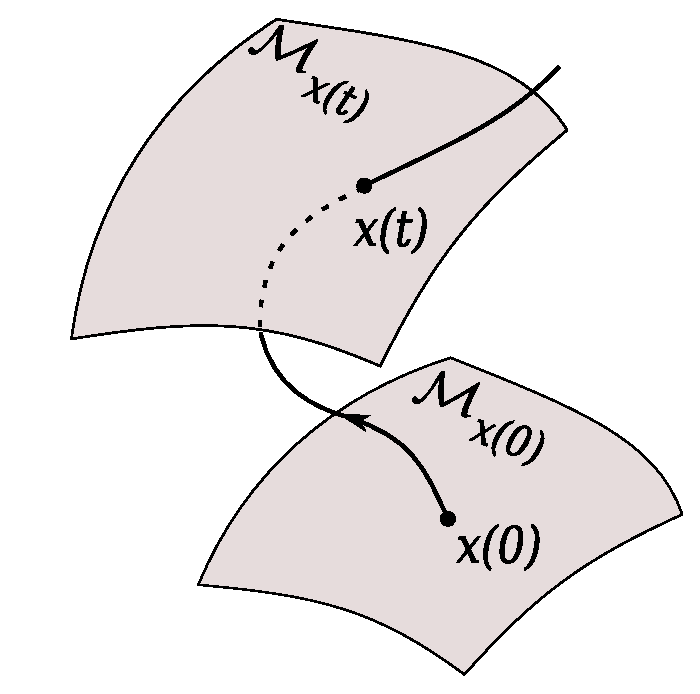
\includegraphics[width=1.00\textwidth,clip=true]{BeThTraj}
 \begin{center}
  \setlength{\unitlength}{1.00\textwidth}
  %% \unitlength = units used in the Picture Environment
  \begin{picture}(1,1.07471658)%
    \put(0,0){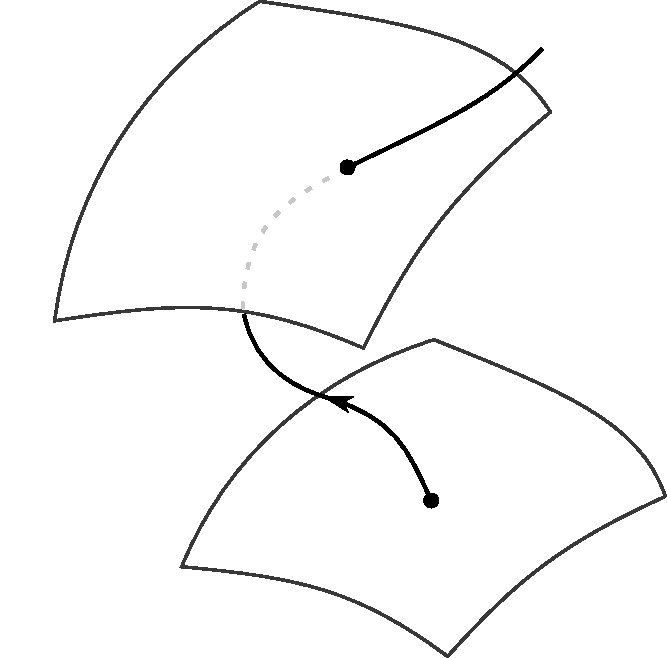
\includegraphics[width=\unitlength]{BeThTrajTeX}}%
    \put(0.28879298,1.02196543){\color[rgb]{0,0,0}\rotatebox{-22.37140782}{\makebox(0,0)[lb]{\smash{$\pS_{\ssp(\tau)}$}}}}%
    \put(0.55566402,0.45078735){\color[rgb]{0,0,0}\rotatebox{-16.6673442}{\makebox(0,0)[lb]{\smash{$\pS_{\ssp(0)}$}}}}%
    \put(0.63028127,0.18433597){\color[rgb]{0,0,0}\rotatebox{0.03136739}{\makebox(0,0)[lb]{\smash{$\ssp(0)$}}}}%
    \put(0.46253394,0.70182304){\color[rgb]{0,0,0}\rotatebox{0.03136739}{\makebox(0,0)[lb]{\smash{$\ssp(\tau)$}}}}%
    \put(0.03852492,0.09250899){\color[rgb]{0,0,0}\rotatebox{0.11031334}{\makebox(0,0)[lb]{\smash{$\pS$}}}}%
  \end{picture}%
 \end{center}
\end{block}
  \column{0.5\textwidth}
		\only<1>{
\noindent
\emph{group orbit} $\pS_\ssp $ of $\ssp$ is the set of all group
actions
\[
\pS_\ssp = \{\LieEl\,\ssp \mid \LieEl \in {\Group}\}
\]
        }
		\only<2>{
%\noindent
%group orbit $\pS_{\ssp(0)}$ of \statesp\ point
% $\ssp(0)$, and the group orbit $\pS_{\ssp(t)}$
%reached by the trajectory $\ssp(t)$ time $t$ later.
%        }
%		\only<3>{
\noindent
any point on the manifold $\pS_{\ssp(t)}$ is
equivalent to any other
        }
		\only<3>{
\noindent
action of a symmetry group
stratifies the \statesp\ into a union of group
orbits

\medskip

each group orbit an equivalence class
        }
\end{columns}
\end{frame}

\section{symmetry reduction}

\begin{frame}{}
\begin{block}{the goal}
replace each group orbit by a unique
point in a lower-dimensional

\bigskip

\hfill
\textcolor{red}{\Large symmetry \reducedsp\ $\pS/\Group$}
\end{block}
\end{frame}

\begin{frame}{symmetry reduction}
  \begin{columns}
  \column{0.5\textwidth}
\begin{block}{full \statesp}
 \begin{center}
  \setlength{\unitlength}{1.00\textwidth}
  %% \unitlength = units used in the Picture Environment
  \begin{picture}(1,1.07315413)%
    \put(0,0){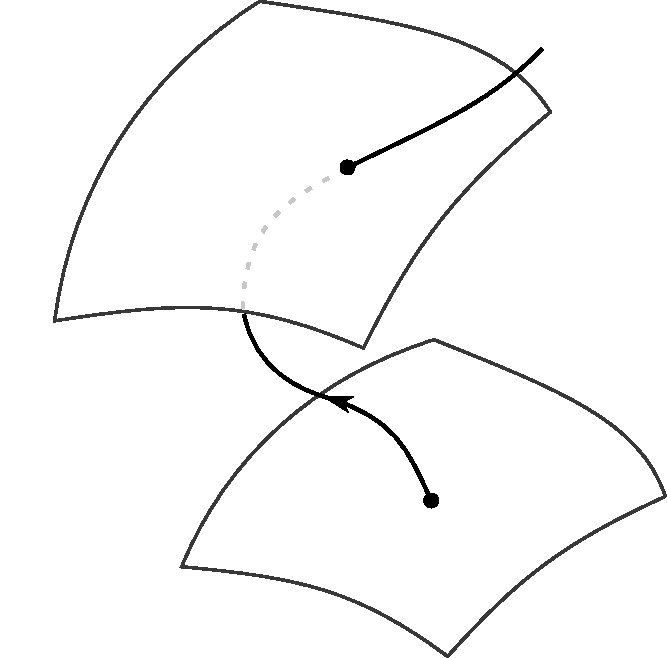
\includegraphics[width=\unitlength]{BeThTrajTeX}}%
    \put(0.30362031,0.99939308){\color[rgb]{0,0,0}\rotatebox{-31.32889204}{\makebox(0,0)[lb]{\smash{$\pS_{\ssp(\tau)}$}}}}%
    \put(0.5686188,0.45975596){\color[rgb]{0,0,0}\rotatebox{-40.8073288}{\makebox(0,0)[lb]{\smash{$\pS_{\ssp(0)}$}}}}%
    \put(0.63028127,0.18433598){\color[rgb]{0,0,0}\rotatebox{0.03136739}{\makebox(0,0)[lb]{\smash{$\ssp(0)$}}}}%
    \put(0.46253394,0.70182305){\color[rgb]{0,0,0}\rotatebox{0.03136739}{\makebox(0,0)[lb]{\smash{$\ssp(\tau)$}}}}%
  \end{picture}%
 \end{center}
\end{block}
  \column{0.5\textwidth}
\begin{block}{\reducedsp}
 \begin{center}
  \setlength{\unitlength}{1.00\textwidth}
  %% \unitlength = units used in the Picture Environment
  \begin{picture}(1,1.07315413)%
    \put(0,0){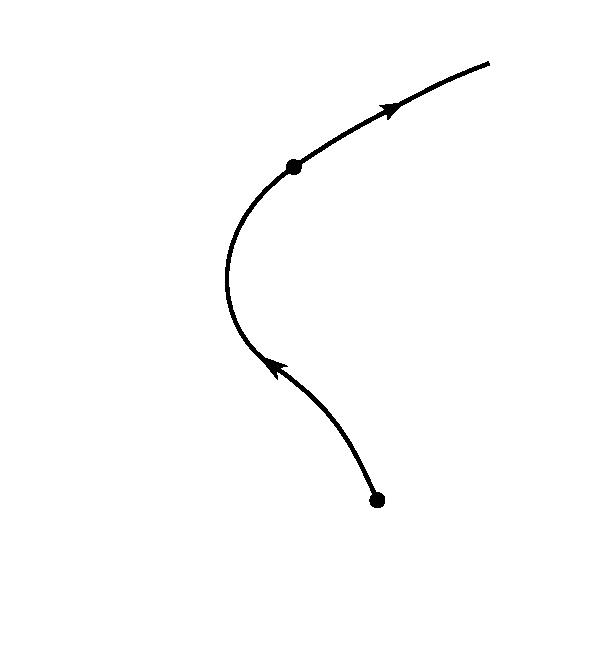
\includegraphics[width=\unitlength]{BeThRedTeX}}%
    \put(0.19912369,0.17144733){\color[rgb]{0,0,0}\rotatebox{0.11031334}{\makebox(0,0)[lb]{\smash{$\pSRed$}}}}%
    \put(0.63028127,0.18433598){\color[rgb]{0,0,0}\rotatebox{0.03136739}{\makebox(0,0)[lb]{\smash{$\sspRed(0)$}}}}%
    \put(0.46253394,0.70182305){\color[rgb]{0,0,0}\rotatebox{0.03136739}{\makebox(0,0)[lb]{\smash{$\sspRed(\tau)$}}}}%
  \end{picture}%
 \end{center}
\end{block}
\end{columns}
\end{frame}


\begin{frame}{pedestrian attempt : \reqv\ or `traveling wave'}
%\includegraphics[width=0.8\textwidth,clip=true]{AW-TW2}

dynamical orbit confined to the group orbit
\[
\LieEl(\tau) \, \ssp(0) =
\ssp(\tau) \in \pS_{\REQV{}{}}
\]
\end{frame}

\begin{frame}{pedestrian${}^*$ attempt : moving frame}
%\includegraphics[width=0.8\textwidth,clip=true]{AW-TW3}

\reqv\ is made stationary by
\\
a counter-rotating `frame'

\end{frame}

\begin{frame}{sophisticate attempt : Faddeev-Popov gauge fixing}
the equivalence principle: integrate over classes of gauge equivalent fields instead
of all fields $A_\mu^a$.

The representative in the class of equivalent fields is
fixed by a gauge condition,
\[
    \partial_{\mu} A_{\mu}^{a} = 0
    \,,
\]
a plane intersected by the gauge orbits
\[
    A_{\mu} = A_{\mu}^{a}t_{a} \to A_{\mu}^{\Omega}
            = \Omega A_{\mu} \Omega^{-1} + \partial_{\mu} \Omega \Omega^{-1} .
\]
abelian orbits intersect the plane at the same angle.
The non-abelian
intersection angle depends on the field.
\end{frame}

\begin{frame}{sophisticate attempt : connections or `gauge fixing'}
%%%%%%%%%%%%%%%%%%%%%%%%%%%%%%%%%%%%%%%%%%%%%%%%%%%%%%%%%%%%%%%%%%%%%
%\label{fig:tangents}
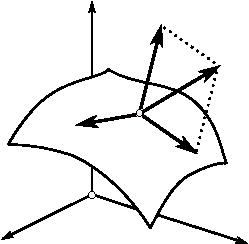
\includegraphics[width=0.40\textwidth]{A28tangents}
2-continuous parameter symmetry: each \statesp\ point
$\ssp$ owns 3 tangent vectors

one $\vel(\ssp)$ along the time flow

two group tangents $\groupTan^{(1)}(\ssp)$, $\groupTan^{(2)}(\ssp)$
along infinitesimal symmetry shifts
%%%%%%%%%%%%%%%%%%%%%%%%%%%%%%%%%%%%%%%%%%%%%%%%%%%%%%%%%%%%%%%%%%%%%

\begin{block}{a flow }
normal to group tangent directions
\end{block}

North Korean gauge : slacking along non-shape-changing directions is
forbidden
\end{frame}


\begin{frame}{sophisticate attempt : connections or `gauge fixing'}
%%%%%%%%%%%%%%%%%%%%%%%%%%%%%%%%%%%%%%%%%%%%%%%%%%%%%%%%%%%%%%%%%%%%%
%\label{fig:tangents}
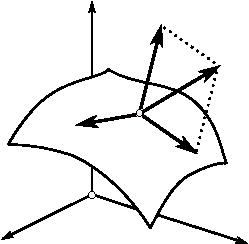
\includegraphics[width=0.40\textwidth]{A28tangents}
2-continuous parameter symmetry: each \statesp\ point
$\ssp$ owns 3 tangent vectors

one $\vel(\ssp)$ along the time flow

two group tangents $\groupTan^{(1)}(\ssp)$, $\groupTan^{(2)}(\ssp)$
along infinitesimal symmetry shifts
%%%%%%%%%%%%%%%%%%%%%%%%%%%%%%%%%%%%%%%%%%%%%%%%%%%%%%%%%%%%%%%%%%%%%

\begin{block}{a flow }
normal to group tangent directions
\end{block}

North Korean gauge : forbid slacking along non-shape-changing directions
\end{frame}

\begin{frame}{method of ``connections''}
%\label{fig:A28extremum}
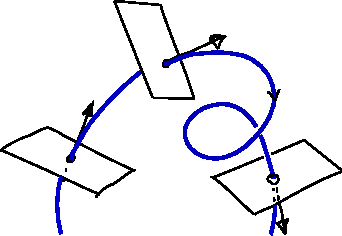
\includegraphics[width=0.60\textwidth]{A28mConnect}

never stray along the group directions, always move orthogonally to
the group orbit
\end{frame}


\section[slice n' dice]{slice n' dice}


\begin{frame}{relativity for cyclists}
\begin{block}{method of moving frames / slices}

\bigskip
cut group orbits by a hypersurface
\textcolor{red}{(not a Poincar\'e section)}, each group orbit of
symmetry-equivalent points represented by the single point
\end{block}
\bigskip
\textcolor{blue}{\Large cut how?}
\end{frame}


\begin{frame}{inspiration: pattern recognition}
you are observing turbulence in a pipe flow, or your defibrillator has a
mesh of sensors measuring electrical currents that cross your heart, and

\medskip

you have a precomputed pattern, and are sifting through the data set of
observed patterns for something like it

\medskip

here you see a pattern, and there you see a pattern that seems much like
the first one

\bigskip

\bigskip

\textcolor{red}{\Large how `much like the first one?'}
\end{frame}

\begin{frame}{}
take the first pattern
\begin{block}{`template' or `reference state'}
\hfill  a point {\slicep} in the \statesp\  \pS
\end{block}

and use the symmetries of the flow to
\begin{block}{slide and rotate the `{\template}'}
\hfill  act with elements of the symmetry group \Group\ on
$\slicep \to \LieEl(\gSpace)\,\slicep$
\end{block}
 until it overlies the second pattern (a point $\ssp$ in
the \statesp)
\begin{block}{distance between the two patterns}
\[ %beq
|\ssp - \LieEl(\gSpace)\,\slicep|
    = |\sspRed - \slicep|
%\label{minDistance}
\] %eeq
\end{block}
is minimized
\end{frame}

\begin{frame}{moving frame}
%\label{fig:A27movFrame}
  \setlength{\unitlength}{0.60\textwidth}
  \begin{picture}(1,0.95956879)%
    \put(0,0){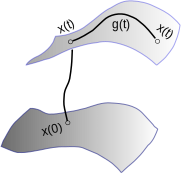
\includegraphics[width=\unitlength]{A27movFrame1}}%
    \put(0.23452859,0.20577397){\color[rgb]{0,0,0}\rotatebox{13.70564637}{\makebox(0,0)[lb]{\smash{$\ssp(0)$}}}}%
    \put(0.33101524,0.7744554){\color[rgb]{0,0,0}\rotatebox{25.42186498}{\makebox(0,0)[lb]{\smash{$\ssp(\zeit)$}}}}%
    \put(0.8633058,0.79722561){\color[rgb]{0,0,0}\rotatebox{-35.54161781}{\makebox(0,0)[lb]{\smash{$\sspRed(\zeit)$}}}}%
    \put(0.61945216,0.80401789){\color[rgb]{0,0,0}\makebox(0,0)[lb]{\smash{$\LieEl(\zeit)$}}}%
  \end{picture}%
\end{frame}

\begin{frame}{idea: the closest match}
%\label{fig:A28extremum}
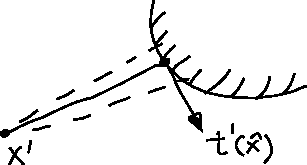
\includegraphics[width=0.60\textwidth]{A28extremum}

extremal condition for nearest distance
\end{frame}

\begin{frame}{idea: the closest match}
  \begin{columns}
  \column{0.60\textwidth}
\begin{block}{} %group orbits}
\begin{center}
  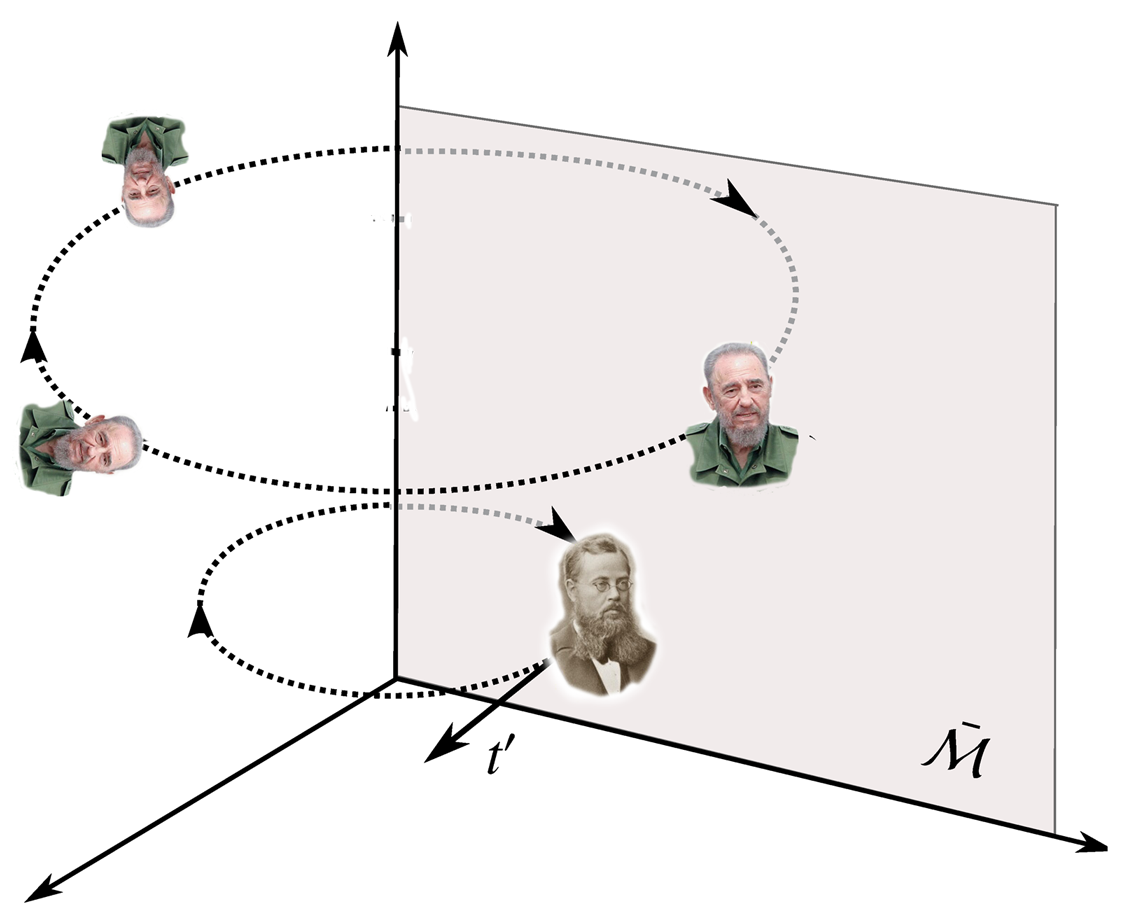
\includegraphics[width=1.00\textwidth,clip=true]
  {sliceLie}
\end{center}
\end{block}
  \column{0.40\textwidth}
template: Sophus Lie

\bigskip
(1) rotate bearded guy $\ssp$
\\
\textcolor{blue}{traces out the group orbit $\pS_\ssp$}

\bigskip
(2) replace the group orbit by the closest match $\sspRed$
to the template pattern $\slicep$

\bigskip
the closest matches $\sspRed$ lie in the $(d\!-\!N)$ symmetry \reducedsp\
$\pSRed$
\end{columns}
\end{frame}

\begin{frame}{distance}
assume that \Group\
is a subgroup of the group of orthogonal transformations
$\On{d}$, and measure
distance $|\ssp|^2=\braket{\ssp}{\ssp}$ in terms of the Euclidean inner
product

\bigskip
numerical fluids:  PDE discretization independent L2 distance is
\begin{block}{energy norm}
\[
  \Norm{\bu-\bv}^2  = \braket{\bu-\bv}{\bu-\bv}  = \frac{1}{V}
                \int_\bCell \! d \bx \;
                       (\bu-\bv) \cdot (\bu-\bv)
%\label{innerproduct}
\]
\end{block}

\bigskip
experimental fluid:
\begin{block}{image discretization independent distance}
 is Hamming distance, or ???
\end{block}
\end{frame}

\subsection{\mslices}

\begin{frame}{}
\begin{block}{minimal distance}
is a solution to the extremum conditions
\[ %beq
\frac{\partial ~~}{\partial \gSpace_a} |\ssp - \LieEl(\gSpace)\,\slicep|^2
\] % ee{PCsectQ0}
\end{block}
\bigskip
but what is
\[
\frac{\partial ~~}{\partial \gSpace_a} \LieEl(\gSpace)
\,?
\]
\end{frame}

\section{slice \& dice}

\subsection[Lie groups]{Lie groups for pedestrians}
% \subsection{Group representations}
% \subsection{Compact groups}
% Predrag                               13 aug 2006
% extracted from GroupTheory webbook
% \Chapter{grint}{August 13, 2006}{Group integrals}

\begin{frame}{Lie algebras for pedestrians}
an element of a compact Lie group:
\[
\LieEl(\gSpace) \propto e^{\gSpace \cdot \Lg }
	\,,\qquad
\gSpace \cdot \Lg  = \sum \gSpace_a \Lg_a,\; a=1,2, \cdots, N
\] %ee{FiniteRot}
$\gSpace \cdot \Lg$: {\em Lie algebra} element
\\
$\gSpace_a$: parameters of the transformation.

\bigskip
\begin{block}{infinitesimal transformations}
\[
g=e^{\delta \gSpace \cdot \Lg}
 \simeq  1 + \gSpace \cdot \Lg \,, \qquad \vert \delta \gSpace \vert \ll 1
\]
\end{block}
\begin{block}{Lie algebra}
\begin{itemize}
  \item $T_a$ are \textcolor{blue}{generators} of infinitesimal
transformations
  \item here $T_a$ are $[d\!\times\!d]$ antisymmetric matrices
  \item $T_a$ are elements of the Lie algebra of $\Group$
\end{itemize}
\end{block}
\end{frame}

\begin{frame}{example: \SOn{2} invariance of \cLe}
\cLe\ equations are invariant under
\\
\SOn{2} rotation by finite angle \gSpace:
\[
\LieEl(\gSpace) \,=\,  \left(\barr{ccccc}
  \cos \gSpace  & \sin \gSpace  & 0 & 0 & 0 \\
 -\sin \gSpace  & \cos \gSpace  & 0 & 0 & 0 \\
 0 & 0 &  \cos \gSpace & \sin \gSpace   & 0 \\
 0 & 0 & -\sin \gSpace & \cos \gSpace   & 0 \\
 0 & 0 & 0             & 0              & 1
    \earr\right)
\] %{CLfRots}
%\begin{frame}{example:
\SOn{2} Lie algebra has one generator
of infinitesimal rotations
\[
 \Lg \,=\,   \left(\barr{ccccc}
    0  &  1 & 0  &  0 & 0  \\
   -1  &  0 & 0  &  0 & 0 \\
    0  &  0 & 0  &  1 & 0  \\
    0  &  0 &-1  &  0 & 0 \\
    0  &  0 & 0  &  0 & 0
    \earr\right)
\] %ee{CLfLieGen}
\end{frame}

\begin{frame}{now have the `slice condition'}
\begin{block}{group tangent fields}
flow field at the \statesp\
point $\ssp$ induced by the action of the group is given by
the set of $N$ \emph{tangent fields}
\[
\groupTan_a(\ssp)_{i}= (\Lg_a){}_{ij} \ssp_j
\] %{GroupTangField}
\end{block}
\bigskip
\begin{block}{slice condition}
\[ %beq
\frac{\partial ~~}{\partial \gSpace_a} |\ssp - \LieEl(\gSpace)\,\slicep|^2
   =
2\, \braket{\sspRed - \slicep}{\sliceTan{a}}
   = 0
    \,,\qquad
	  \sliceTan{a} = \Lg_a \slicep
\] % ee{PCsectQ0}
\end{block}
\end{frame}

\begin{frame}{flow within the slice}
\slice\ fixed by \slicep

\bigskip
	\begin{exampleblock}
          {\reducedsp\ $\pSRed$  flow $\velRed(\sspRed)$}
\bea
\velRed(\sspRed) &=& \vel(\sspRed)
                    \,-\, \dot{\gSpace}(\sspRed)  \cdot \groupTan(\sspRed)
    \,,\qquad\quad \sspRed \in \pSRed
\continue
\dot{\gSpace}_a(\sspRed) &=& (\vel(\sspRed)^T \sliceTan{a})
                       /(\groupTan(\sspRed)^T \cdot \sliceTan{})
\,.
\nnu %\label{EqMotMFrame}
\eea
	\end{exampleblock}
\begin{itemize}
  \item $\vel$ : velocity, full space
  \item $\velRed$ : velocity component in slice
  \item $\dot{\gSpace}  \cdot \groupTan$ : velocity component normal to slice
  \item $\dot{\gSpace}$ : reconstruction equation for the group phases
\end{itemize}
\begin{block}{Cartan derivative}
\[
\LieEl^{-1}\dot{\LieEl} \,\ssp
    =e^{-\gSpace \cdot \Lg} \,
\frac{d ~~}{d \, \tau} e^{\gSpace \cdot \Lg}\ssp
    =\dot{\gSpace}\cdot \groupTan(\ssp)
\]
\end{block}
\end{frame}

\begin{frame}{flow within the slice}
\begin{block}{} %group orbits}
\begin{center}
  \includegraphics[width=0.70\textwidth,clip=true]
  {sliceRaw}
\end{center}
\end{block}
full-space trajectory $\ssp(\tau)$ \\
rotated into the \reducedsp\ $\sspRed(\tau) = \LieEl(\gSpace)^{-1}\ssp(\tau)$ \\
by appropriate \emph{moving frame} angles $\{\gSpace(\tau)\}$
\end{frame}

\begin{frame}{\rpo}
a \rpo\ $p$ is an orbit in
{\statesp} $\pS$ which exactly recurs
%    \PC{create SFIG here}
\beq
\ssp_p (t) = g_p \ssp_p (t + \period{p} )
    \,,\qquad
\ssp_p (t) \in \pS_p
\label{RPOrelper1}
\eeq
for a fixed \textcolor{blue}{relative period} $\period{p}$
and a fixed group action ${g_p} \in  \Group$
that ``rotates" the endpoint $\ssp_p (\period{p} ) $
back into the initial point $\ssp_p (0) $.
\end{frame}

\begin{frame}{\rpo $\to$ \po}
%%%%%%%%%%%%%%%%%%%%%%%%%%%%%%%%%%%%%%%%%%%%%%%%%%%%%%%%%%%%%%%%
%% slice.*, inflectHype.*: see dasbuch/book/FigSrc/inkscape/00ReadMe.txt
%% rpo.* hand-drawn in dasbuch/book/FigSrc/xfig/rpo.fig
%% xfig exported -> FigSrc/inkscape/rpo.fig
%% inkscape exported -> rpo.eps + LaTeX, hand edited in the macros
%% Predrag 2011-08-27 replaced rpo.pdf by rpoSlice.pdf
%%  2011-09-09 Predrag: updated continuous.tex overheads
%% remember to insert rpoSlice.pdf into ChaosBook
\begin{block}{}
 \begin{center}
  \setlength{\unitlength}{0.70\textwidth}
  %% \unitlength = units used in the Picture Environment
  \begin{picture}(1,0.87085079)%
    \put(0,0){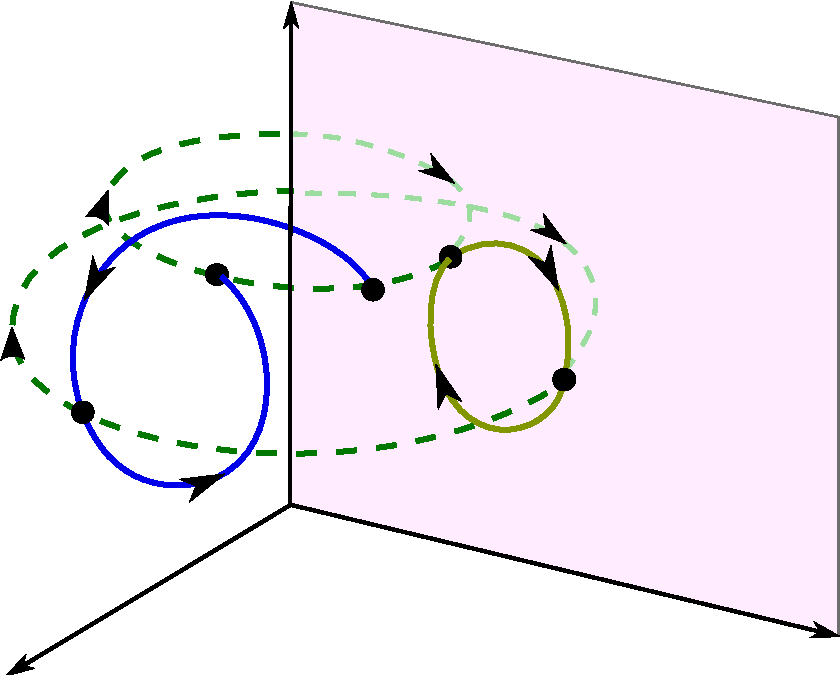
\includegraphics[width=\unitlength]{rpoSlice}}%
    \put(0.82835153,0.19007656){\color[rgb]{0,0,0}\rotatebox{-14.84025432}{\makebox(0,0)[lb]{$\pSRed$}}}%
    \put(0.40925459,0.45713857){\color[rgb]{0,0,0}\rotatebox{0.0313674}{\makebox(0,0)[lb]{\smash{$\ssp(0)$}}}}%
    \put(0.71354118,0.39765314){\color[rgb]{0,0,0}\rotatebox{0.0313674}{\makebox(0,0)[lb]{\smash{$\sspRed(\tau)$}}}}%
    \put(0.13171187,0.38813817){\color[rgb]{0,0,0}\rotatebox{0.0313674}{\makebox(0,0)[lb]{\smash{$\LieEl(\tau)$}}}}%
    \put(0.02168739,0.31359574){\color[rgb]{0,0,0}\rotatebox{0.0313674}{\makebox(0,0)[lb]{\smash{$\ssp(\tau)$}}}}%
    \put(0.15576193,0.48769256){\color[rgb]{0,0,0}\rotatebox{0.0313674}{\makebox(0,0)[lb]{\smash{$\ssp(\period{})$}}}}%
    \put(0.54113911,0.50476963){\color[rgb]{0,0,0}\rotatebox{0.0313674}{\makebox(0,0)[lb]{\smash{$\sspRed(0)$}}}}%
  \end{picture}%
 \end{center}
\end{block}
full \statesp\ \rpo\ $\ssp(\tau)$ \\
is rotated into the \reducedsp\ {\po}
\end{frame}

\begin{frame}{relativity for pedestrians}
		\only<1>{
\begin{block}{in full \statesp}
        }
		\only<2>{
\begin{block}{in \slice}
        }
\begin{center}
		\only<1>{
(\textit{a})
  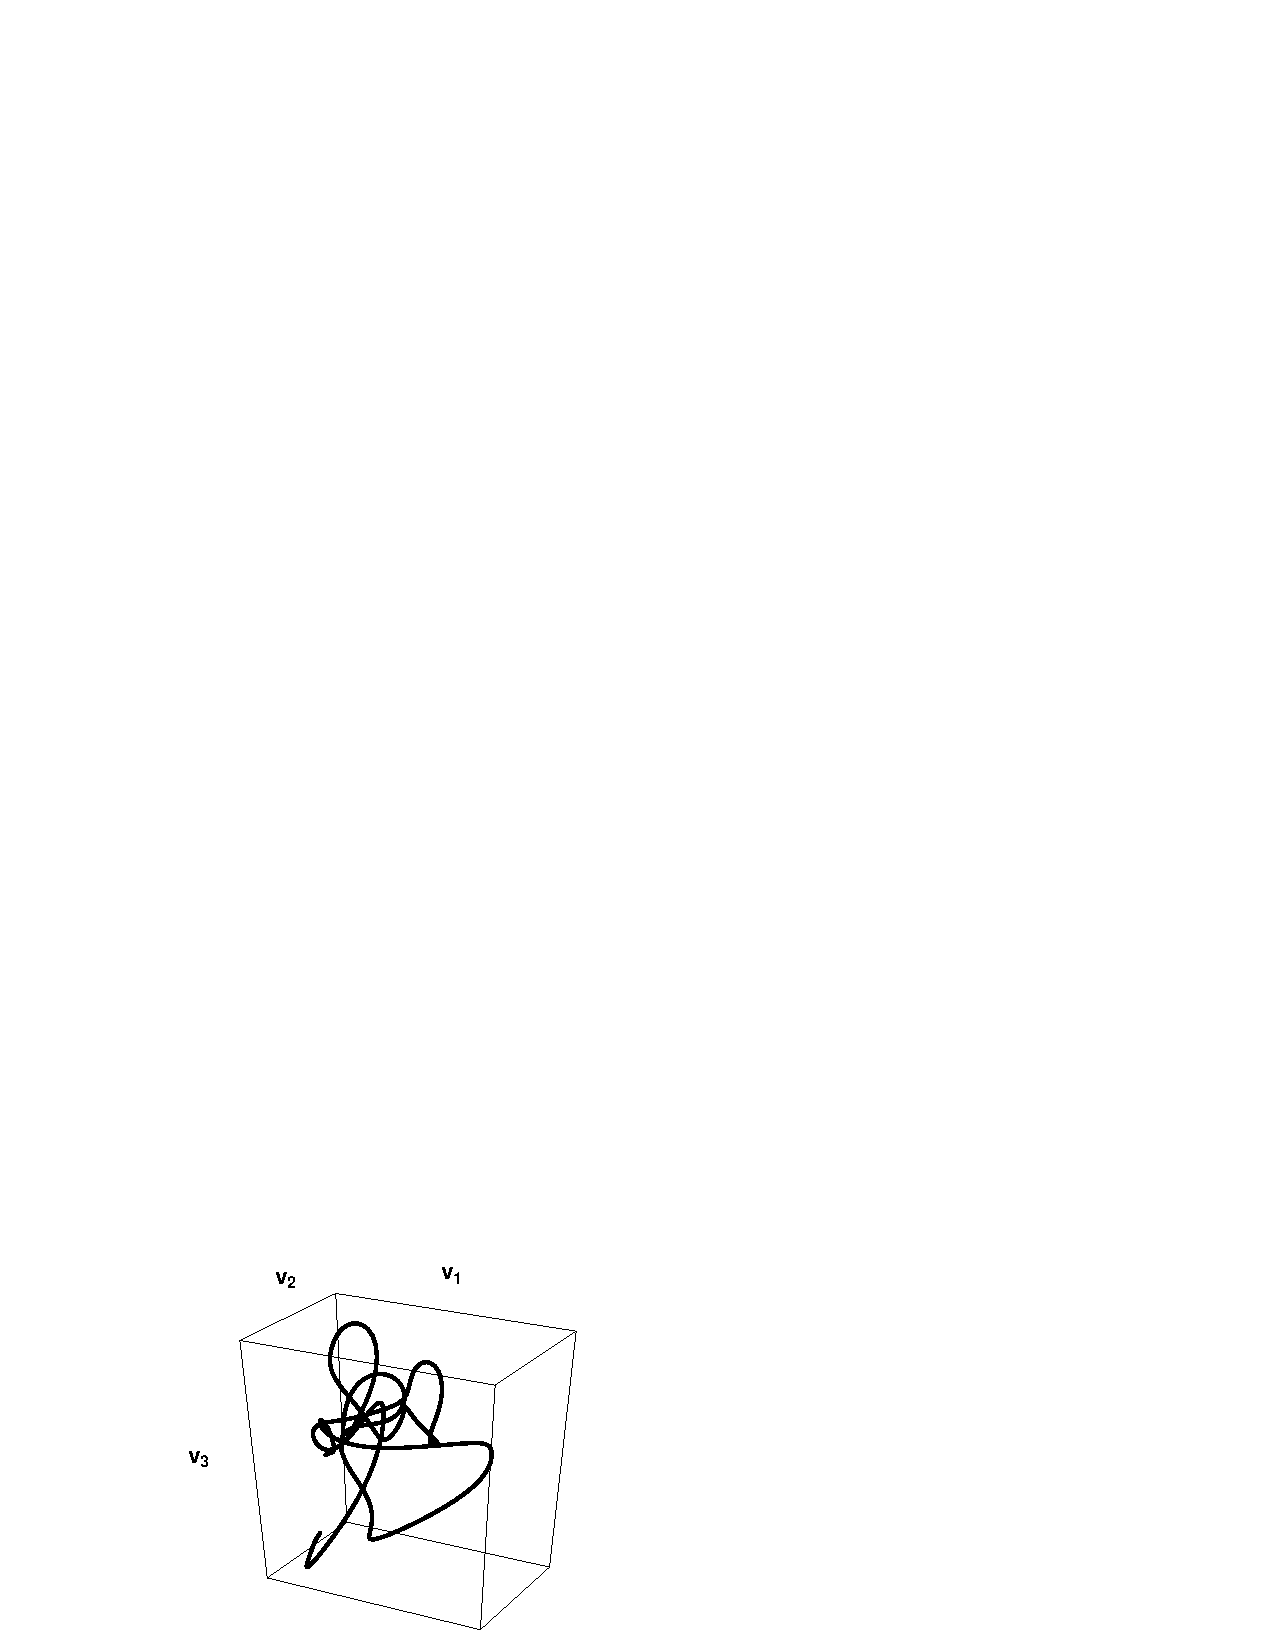
\includegraphics[width=0.40\textwidth,height=0.5\textheight,clip=true]
  {ks22rpo033p50_04p045E2}
        }
		\only<2>{
(\textit{b})
  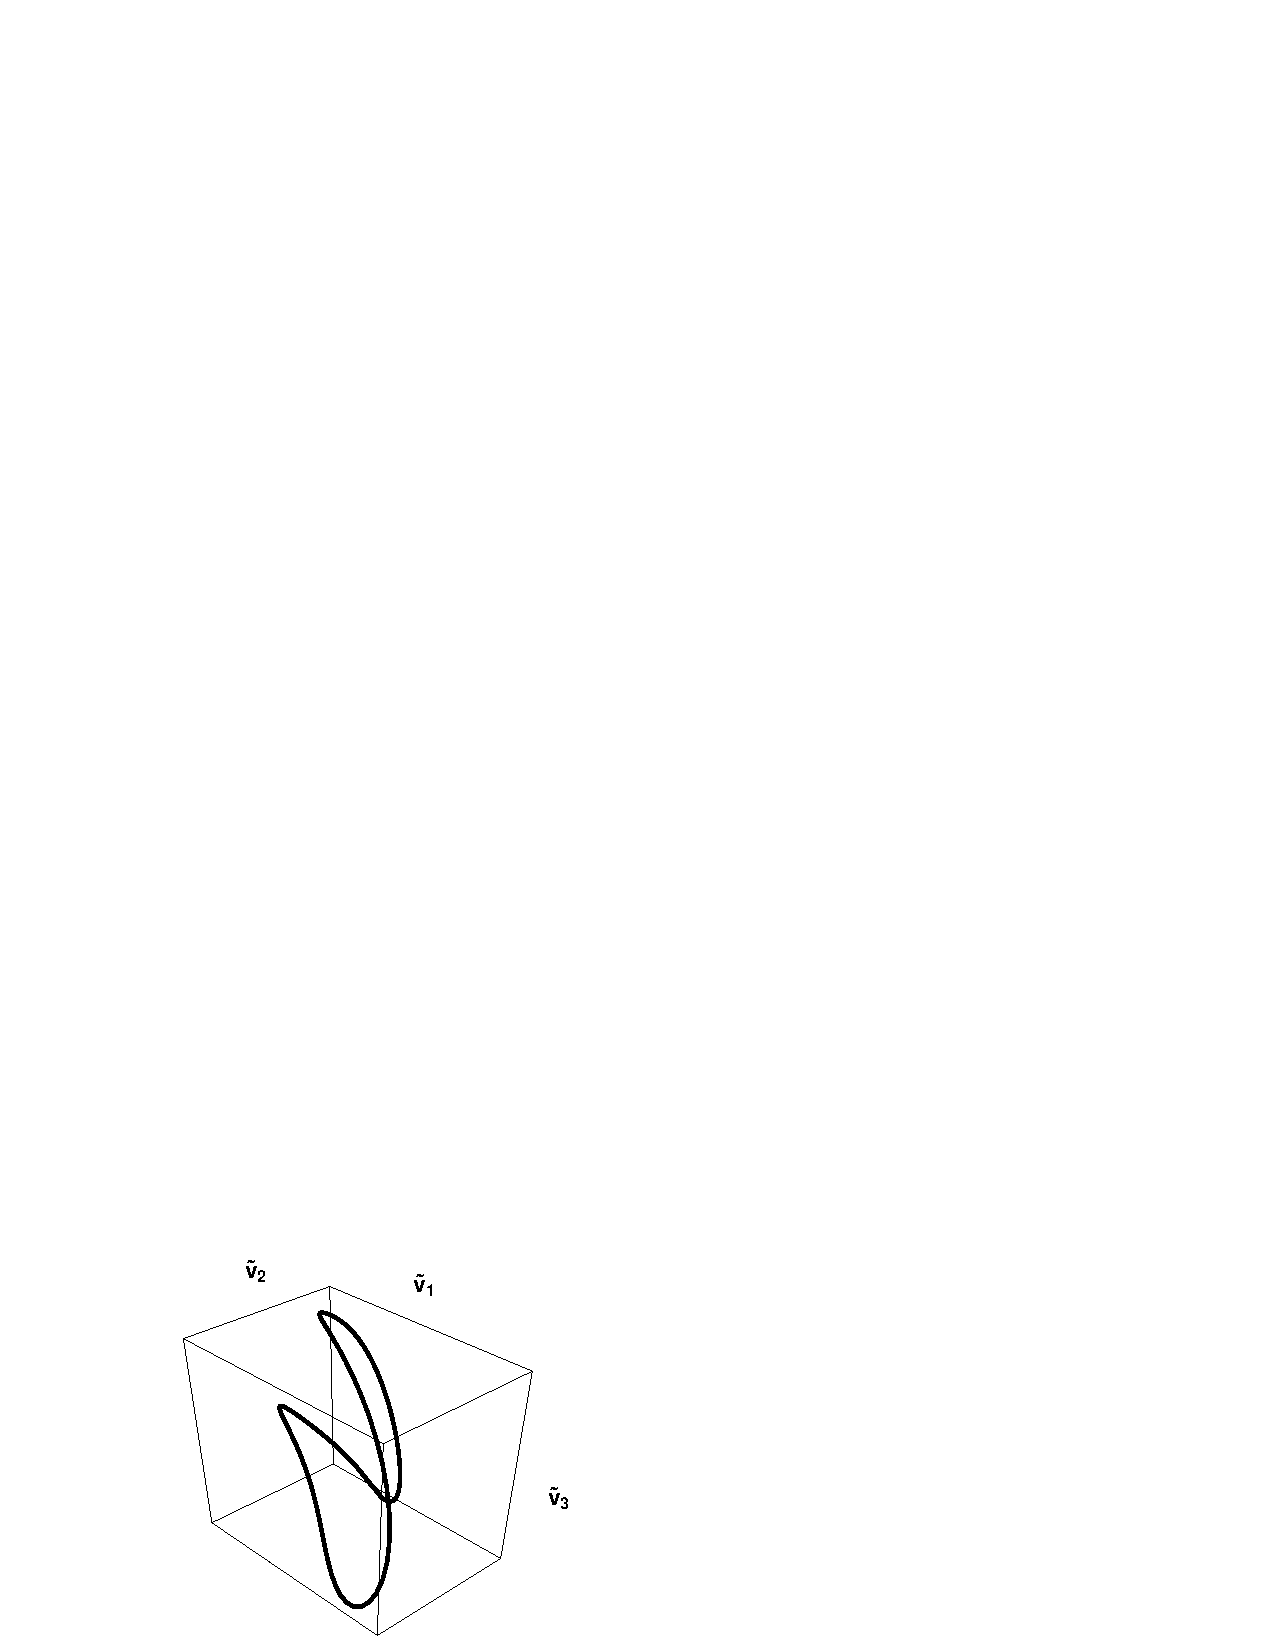
\includegraphics[width=0.40\textwidth,height=0.5\textheight,clip=true]
  {ks22rpo033p50_04p045E2CM}
        }
\end{center}
\end{block}
		\only<1>{
a \rpo\ of the Kuramoto-Sivashinsky flow, 128$d$ \statesp\
traced for four periods
 $\period{p}$, projected on

\bigskip
full \statesp\ coordinate frame
 $\{v_1,v_2,v_3\}$; a mess
        }
		\only<2>{
a \rpo\ of the Kuramoto-Sivashinsky flow projected on

\bigskip
a slice $\{\tilde{v}_1,\tilde{v}_2,\tilde{v}_3\}$ frame
        }
\end{frame}

\begin{frame}{symmetry reduction achieved!}
\begin{itemize}
 \item all points equivalent by symmetries are represented by
    \begin{itemize}
 \item a single point
    \end{itemize}
 \item families of solutions are mapped to a single solution
    \begin{itemize}
 \item \reqva\ become \eqva
 \item \rpo s become \po s
    \end{itemize}
\end{itemize}
\end{frame}

\begin{frame}{take-home message}
rotation into a slice \textcolor{red}{is not} an average\\
 over 3D pipe azimuthal angle

\bigskip\bigskip
it is the full snapshot of the flow embedded in the

\begin{center}
\textcolor{red}{\Large $\infty$-dimensional \statesp}
\end{center}

\bigskip\bigskip
\textcolor{red}{\Large NO information} is lost by symmetry reduction
\begin{itemize}
  \item not modeling by a few degrees of freedom
  \item no dimensional reduction
\end{itemize}
\end{frame}


\begin{frame}{\Large die L\"osung : \cLf\ reduced}
	\begin{columns}[t]
	\column{.50\textwidth}
 		\begin{exampleblock}{full \statesp}
        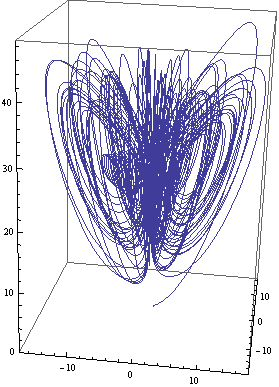
\includegraphics[width=0.7\textwidth,clip=true]
                        {CLEx1x2z} %CLEx1x2zRelEqu}
		\end{exampleblock}
	\column{.50\textwidth}
 		\begin{exampleblock}{\reducedsp}
        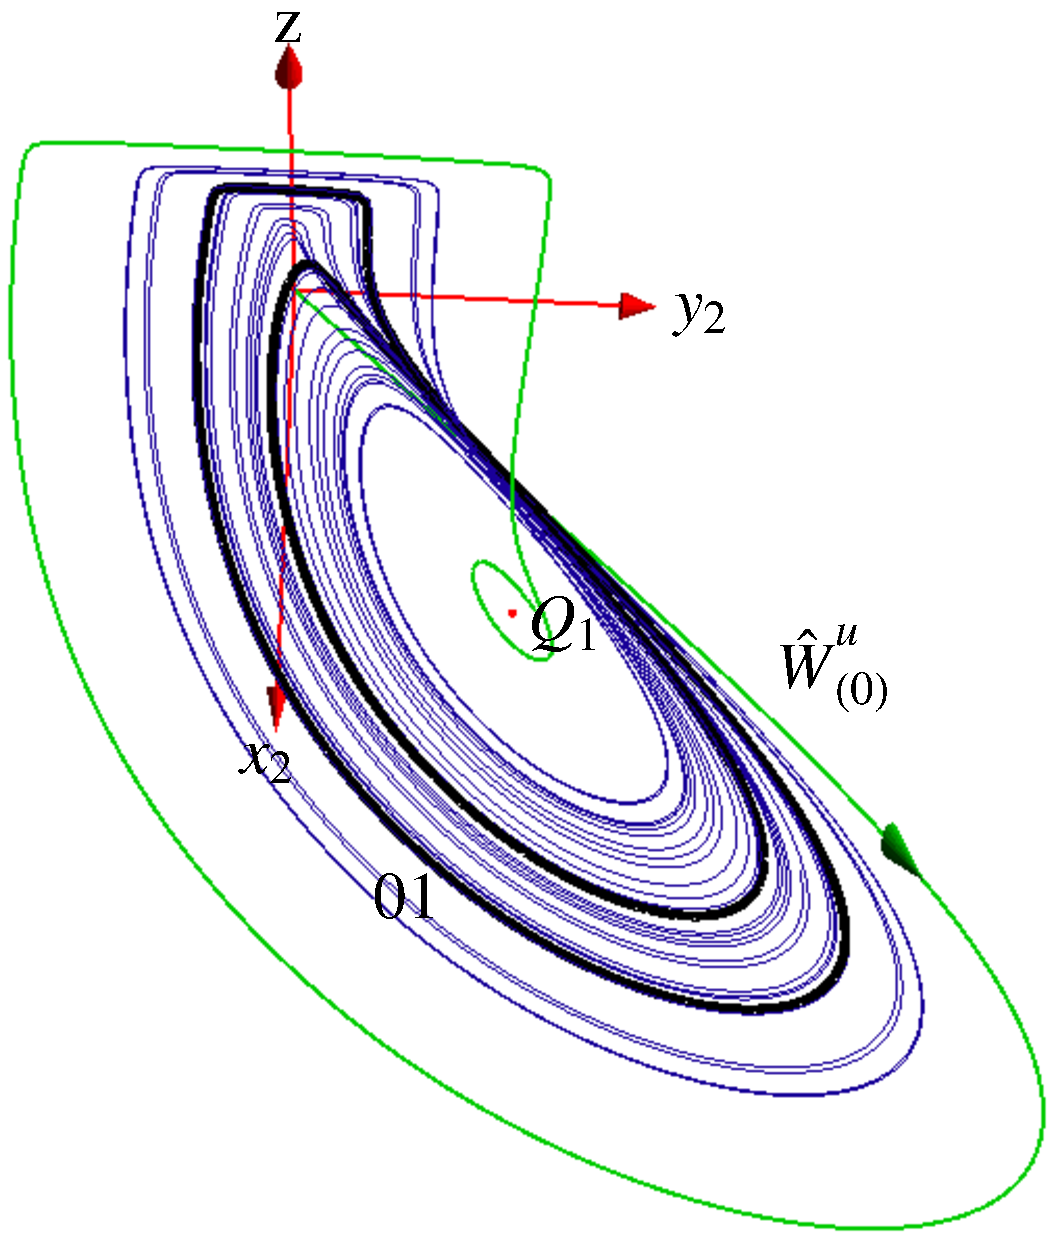
\includegraphics[width=0.6\textwidth,clip=true]
                        {CLEcoord245}
		\end{exampleblock}
	\end{columns}

\bigskip
ergodic trajectory was a mess, now the
topology is reveled
\\
\rpo\ \cycle{01} now a \po
\end{frame}

\begin{frame}{slice trouble 1}
\begin{block}{portrait of \cLf\ in \reducedsp}
\begin{center}
(\textit{a})
  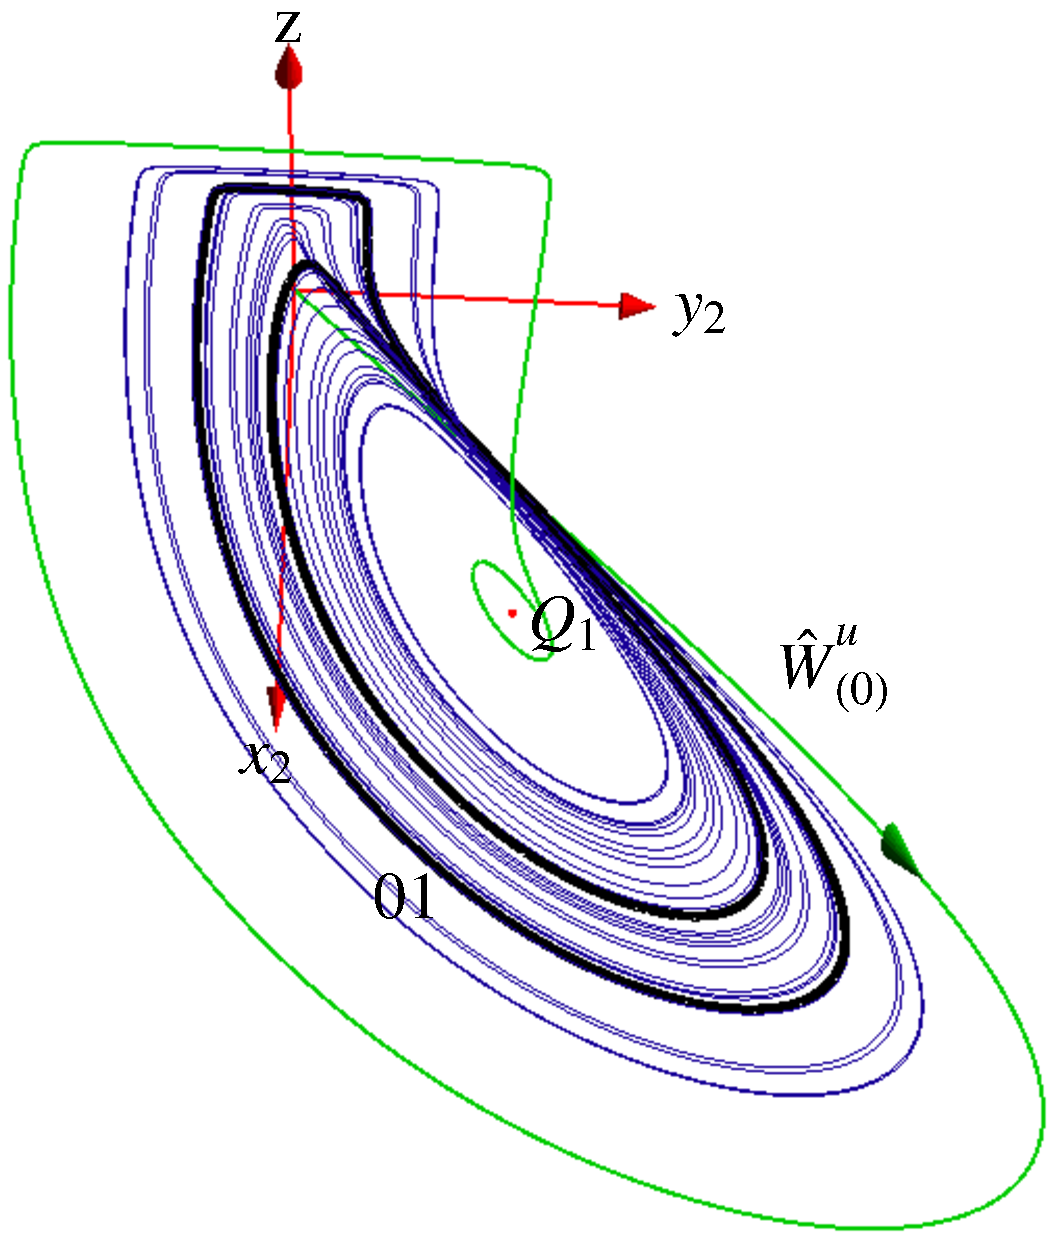
\includegraphics[width=0.40\textwidth,clip=true]
  {CLEcoord245}
(\textit{b})
  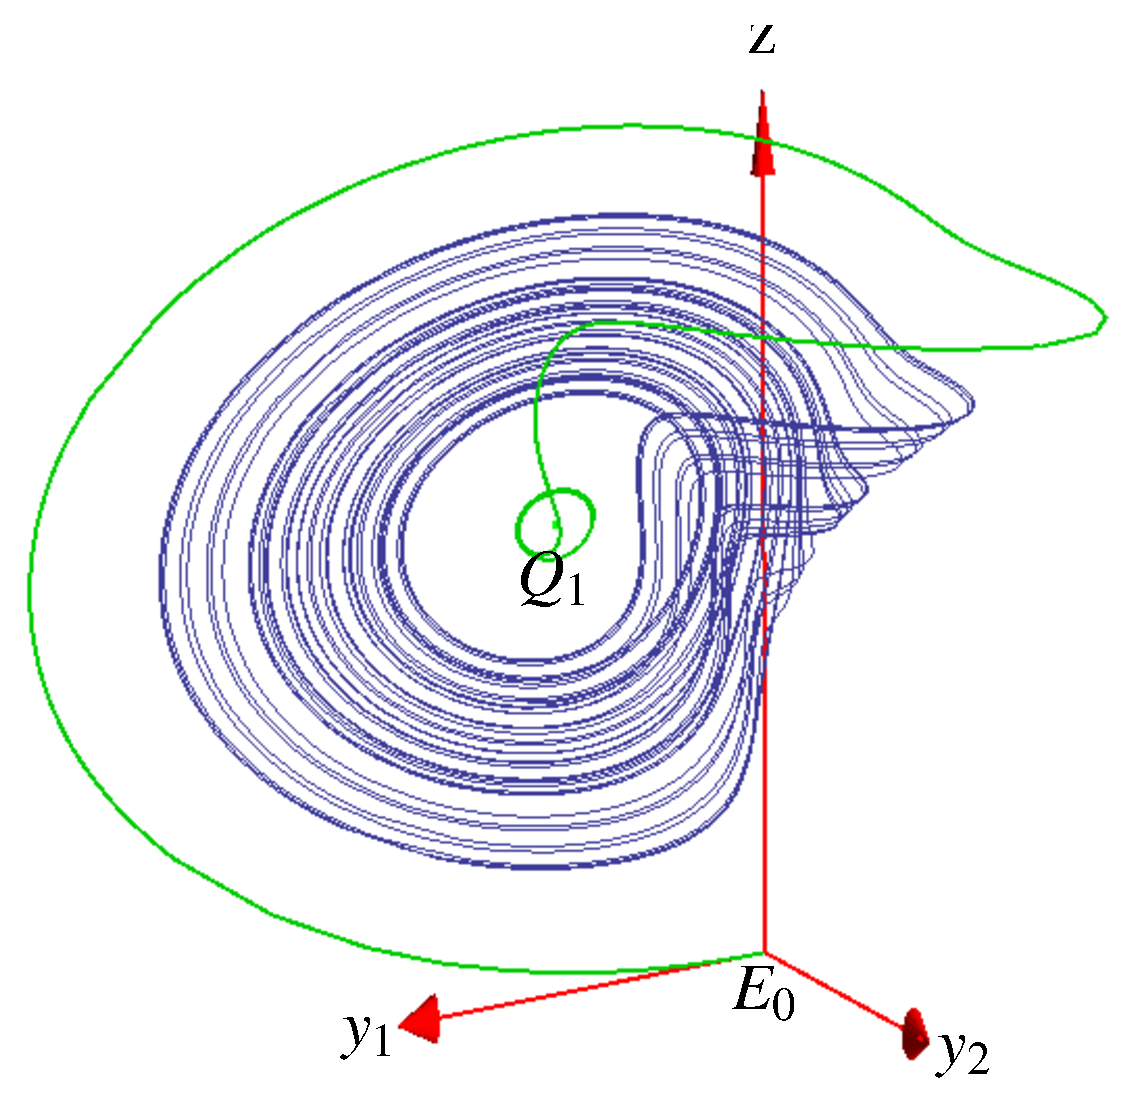
\includegraphics[width=0.45\textwidth,clip=true]
  {CLEperpReqb}
\end{center}
\end{block}
any choices of the slice $\slicep$
exhibit flow discontinuities
\end{frame}

\begin{frame}{slice trouble 1}
\begin{block}{glitches!}
group tangent of a generic trajectory orthogonal
to the slice tangent at a sequence of instants $\tau_k$
\[
\groupTan(\tau_k)^T \cdot \sliceTan{} = 0
\]
\end{block}
\end{frame}

\begin{frame}{example: group orbit of a pipe flow turbulent state}
a turbulent state
%\slicep\ is Kerswell \emph{et al} $N2\_M1$  \reqv\
%( $\Reynolds =2400$, stubby $L=2.5D$ pipe)
	\begin{columns}[t]
	\column{.45\textwidth}
			\begin{exampleblock}
{$\SOn{2}\times\SOn{2}$ symmetry
\\
$\Rightarrow$
group orbit is 2-torus}
			\end{exampleblock}
\begin{block}{distance extremum condition}
$$ %beq
\frac{\partial ~~}{\partial \gSpace_a} |\ssp - \LieEl(\gSpace)\,\slicep|^2
   = 0
$$ % ee{PCsectQ0}
\end{block}
	\column{0.55\textwidth}
\begin{block}
  \centering
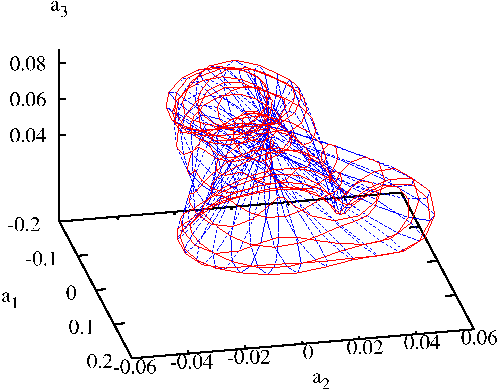
\includegraphics[width=1.00\textwidth]{2840GOt135M1} %{2830GO7}
%  \caption{\label{fig:2830GO6}
    %\label{fig:M1groupOrb}
\end{block}
	\end{columns}

\bigskip
group orbits of highly nonlinear states are highly contorted:
many extrema, multiple sections by a slice
\end{frame}

\begin{frame}{sliced wurst}
a slice hyperplane cuts every group orbit at least twice
 \begin{columns}
 \column{0.4\textwidth}
\begin{block}{slice}
\begin{center}
%\label{fig:sliceimage}
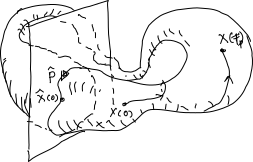
\includegraphics[width=1.00\textwidth]{A29sliceWurst}
\end{center}
\end{block}
 \column{0.6\textwidth}
      an $\SOn{2}$ \rpo\ is topologically a torus : the cuts are \po\
      images of the same \rpo, the good close one, and the rest bad ones
  \end{columns}
\end{frame}

\section{charting the \statesp}

\begin{frame}{trouble: slices cannot be global}
  \begin{columns}
  \column{0.70\textwidth}
\begin{block}{} %group orbits}
\begin{center}
  \includegraphics[width=1.00\textwidth,clip=true]
  {slicePhil}
\end{center}
\end{block}
  \column{0.30\textwidth}
representing a group orbit by the closest match
to a good template $\slicep$
(Phil Morrison)
\end{columns}
\end{frame}

\begin{frame}{trouble: slices cannot be global}
  \begin{columns}
  \column{0.70\textwidth}
\begin{block}{} %group orbits}
\begin{center}
  \includegraphics[width=1.00\textwidth,clip=true]
  {slicePhilY}
\end{center}
\end{block}
  \column{0.30\textwidth}
the `closest match'
to a bad template $\slicep$
(young Phil Morrison) can be a mismatch

\bigskip

\noindent
\textcolor{blue}{single template cannot be a good match  globally}
\end{columns}
\end{frame}

\begin{frame}{trouble: slices cannot be global}
  \begin{columns}
  \column{0.70\textwidth}
\begin{block}{} %group orbits}
\begin{center}
  \includegraphics[width=1.00\textwidth,clip=true]
  {slicePhil0}
\end{center}
\end{block}
  \column{0.30\textwidth}
another attempt, another bad template $\slicep$
(younger Morrison)
\end{columns}
\end{frame}

\begin{frame}{trouble: slices cannot be global}
  \begin{columns}
  \column{0.70\textwidth}
\begin{block}{} %group orbits}
\begin{center}
  \includegraphics[width=1.00\textwidth,clip=true]
  {sliceSonya}
\end{center}
\end{block}
  \column{0.30\textwidth}
representing a group orbit by the closest match
to a better template $\slicep$
(Sonya Kovalewskaya)

\bigskip

\noindent
\textcolor{blue}{to cover $\pS/\Group$ globally, need}:
\\
a set of templates:
\\\begin{itemize}
    \item 2 rolls
    \item 4 rolls
    \item ...
  \end{itemize}
\end{columns}
\end{frame}

\begin{frame}{How good is your slice?}
hyperplane of points \sspSing\ defined by being normal to  the quadratic
Casimir-weighted vector $\Lg^2\slicep$, such that from the {\template}
vantage point their group orbits are not transverse, but locally
`horizontal,'
\[ %beq
\braket{\groupTan(\sspSing)}{\sliceTan{}}
 =
-\braket{\sspSing}{\Lg^2\slicep}
 =0
%\,.
\] %ee{sliceSingl0}
{\scriptsize
(for simplicity, specialize to the  $\SOn{2}$ case)
}
\end{frame}

\begin{frame}{\sset}
%$(d\!-\!2)$\dmn\
$S$ : set of all points $\sspRSing$ which are both
\begin{itemize}
  \item[(a)] in the {\slice}
  \item[(b)] whose group tangent $\groupTan(\sspRSing)$
                is also in the  {\slice}
\end{itemize}
\bea
\braket{\sspRSing}{\sliceTan{}}&=&0 \continue
\braket{\groupTan(\sspRSing)}{\sliceTan{}}
 &=&
-\braket{\sspRSing}{\Lg^2\slicep}
 =0
% \,.
\nnu %label{sliceSingl}
\eea
$S$ is the locus of
inflection points, a hyperplane through which
\begin{itemize}
  \item curvature of the distance function changes sign
  \item local minimum turns into a local maximum
\end{itemize}
\end{frame}

\begin{frame}{\slice\ is good up to \sset}
\begin{block}{}
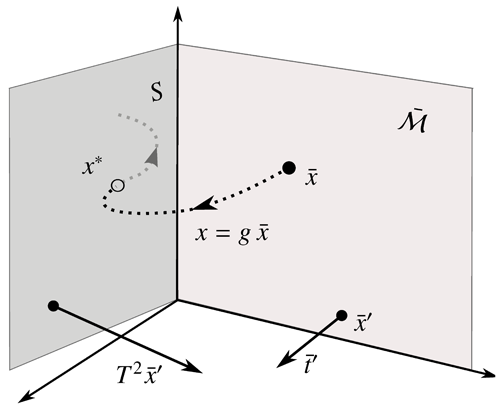
\includegraphics[width=0.80\textwidth]{inflectHype.png}
\end{block}
\end{frame}


\begin{frame}{charting the \statesp}
for turbulent/chaotic systems a set of \Poincare sections is needed to
capture the dynamics. The choice of sections should reflect the
dynamically dominant patterns seen in the solutions of nonlinear PDEs

\medskip

we propose to construct a global atlas of the dimensionally \reducedsp\
$\pSRed$ by deploying linear \Poincare sections $\PoincS{}^{(j)}$ across
neighborhoods of the qualitatively most important patterns $\slicep{}^{(j)}$
\end{frame}

\begin{frame}{2-chart atlas}
%\label{fig:A29-2slices}
  \setlength{\unitlength}{0.80\textwidth}
  %% \unitlength = units used in the Picture Environment
  \begin{picture}(1,0.58916866)%
    \put(0,0){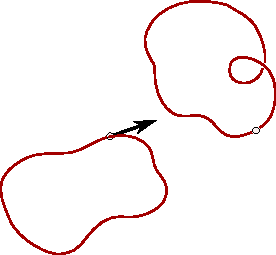
\includegraphics[width=\unitlength]{A29-2tmplts}}%
    \put(0.27072726,0.21951459){\color[rgb]{0,0,0}\makebox(0,0)[lb]{\smash{$\slicep{}^{(1)}$}}}%
    \put(0.65414286,0.27716186){\color[rgb]{0,0,0}\makebox(0,0)[lb]{\smash{$\slicep{}^{(2)}$}}}%
    \put(0.4587488,0.11915476){\color[rgb]{0,0,0}\makebox(0,0)[lb]{\smash{$\sliceTan{}{}^{(1)}$}}}%
    \put(0.49341797,0.44034775){\color[rgb]{0,0,0}\makebox(0,0)[lb]{\smash{$\sliceTan{}{}^{(2)}$}}}%
    \put(0.85958113,0.04536315){\color[rgb]{0,0,0}\makebox(0,0)[lb]{\smash{$\ssp'{}^{(2)}$}}}%
  \end{picture}%

templates $\slicep{}^{(1)}$, $\ssp'{}^{(2)}$, with
group orbits. Start with the {\template} $\slicep{}^{(1)}$. All group
orbits traverse its $(d\!-\!1)$\dmn\ slice hyperplane, including the
group orbit of the second {\template} $\ssp'{}^{(2)}$. Replace the second
{\template} by its closest group-orbit point $\slicep{}^{(2)}$, \ie, the
point in \slice\ $\pSRed{}^{(1)}$.
\end{frame}

\begin{frame}{2-chart atlas}
%\label{fig:A29-2slices}
  \setlength{\unitlength}{0.80\textwidth}
  %% \unitlength = units used in the Picture Environment
  \begin{picture}(1,0.86567815)%
    \put(0,0){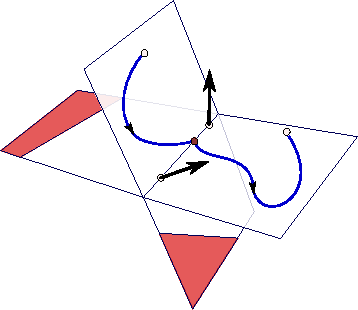
\includegraphics[width=\unitlength]{A29-2slices}}%
    \put(0.3850416,0.38725438){\color[rgb]{0,0,0}\makebox(0,0)[lb]{\smash{$\slicep{}^{(1)}$}}}%
    \put(0.60194012,0.48012421){\color[rgb]{0,0,0}\makebox(0,0)[lb]{\smash{$\slicep{}^{(2)}$}}}%
    \put(0.4042968,0.74412842){\color[rgb]{0,0,0}\makebox(0,0)[lb]{\smash{$\sspRed(0)$}}}%
    \put(0.79647438,0.54627847){\color[rgb]{0,0,0}\makebox(0,0)[lb]{\smash{$\sspRed(\zeit)$}}}%
  \end{picture}%

Now that the group orbits have been reduced to points, consider the two
slices through the two {\template s}. As these two {\template s} are the
closest points viewed from either group orbit, they lie in both \slice s.
However, the two tangent vectors $\sliceTan{}{}^{(1)}$ and
$\sliceTan{}{}^{(2)}$ have different orientations, so they define two
distinct \slice\ hyperplanes $\pSRed{}^{(1)}$ and $\pSRed{}^{(2)}$ which
intersect in the \emph{ridge}, a hyperplane of dimension $(d\!-\!2)$
(here drawn as a `line') shared by the template pair. The chart for the
neighborhood of each template (a page of the atlas on the right side of
the figure) extends only as far as this ridge. If the templates are
sufficiently close, the {\chartBord} of each \slice\ (red region) is
beyond this ridge, and never encountered by the symmetry-reduced
trajectory $\sspRed(\zeit)$. The reduced trajectory is continuous in the
slice comprised of such charts - it switches the chart whenever it
crosses a ridge.
\end{frame}

\begin{frame}{2-chart atlas}
%\label{fig:A29-2slices}
  \setlength{\unitlength}{0.80\textwidth}
  \begin{picture}(1,0.5127804)%
    \put(0,0){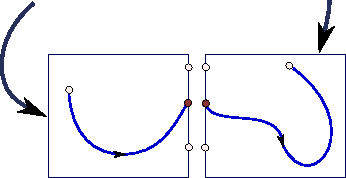
\includegraphics[width=\unitlength]{A29-2charts.pdf}}%
    \put(0.16199231,0.03841546){\color[rgb]{0,0,0}\makebox(0,0)[lb]{\smash{$\pSRed{}^{(1)}$}}}%
    \put(0.63051777,0.0374085){\color[rgb]{0,0,0}\makebox(0,0)[lb]{\smash{$\pSRed{}^{(2)}$}}}%
    \put(0.21517269,0.28787637){\color[rgb]{0,0,0}\makebox(0,0)[lb]{\smash{$\sspRed(0)$}}}%
    \put(0.75921701,0.25014044){\color[rgb]{0,0,0}\makebox(0,0)[lb]{\smash{$\sspRed(\zeit)$}}}%
    \put(0.60952792,0.26511997){\color[rgb]{0,0,0}\makebox(0,0)[lb]{\smash{$\slicep{}^{(2)}$}}}%
    \put(0.45827029,0.02997228){\color[rgb]{0,0,0}\makebox(0,0)[lb]{\smash{$\slicep{}^{(1)}$}}}%
  \end{picture}%

The slice (unique point for each group orbit) is now covered by an atlas
consisting of $(d\!-\!1)$\dmn\ charts $\pSRed{}^{(1)}, \pSRed{}^{(2)},
\cdots$
\end{frame}


\begin{frame}{}
\begin{center}
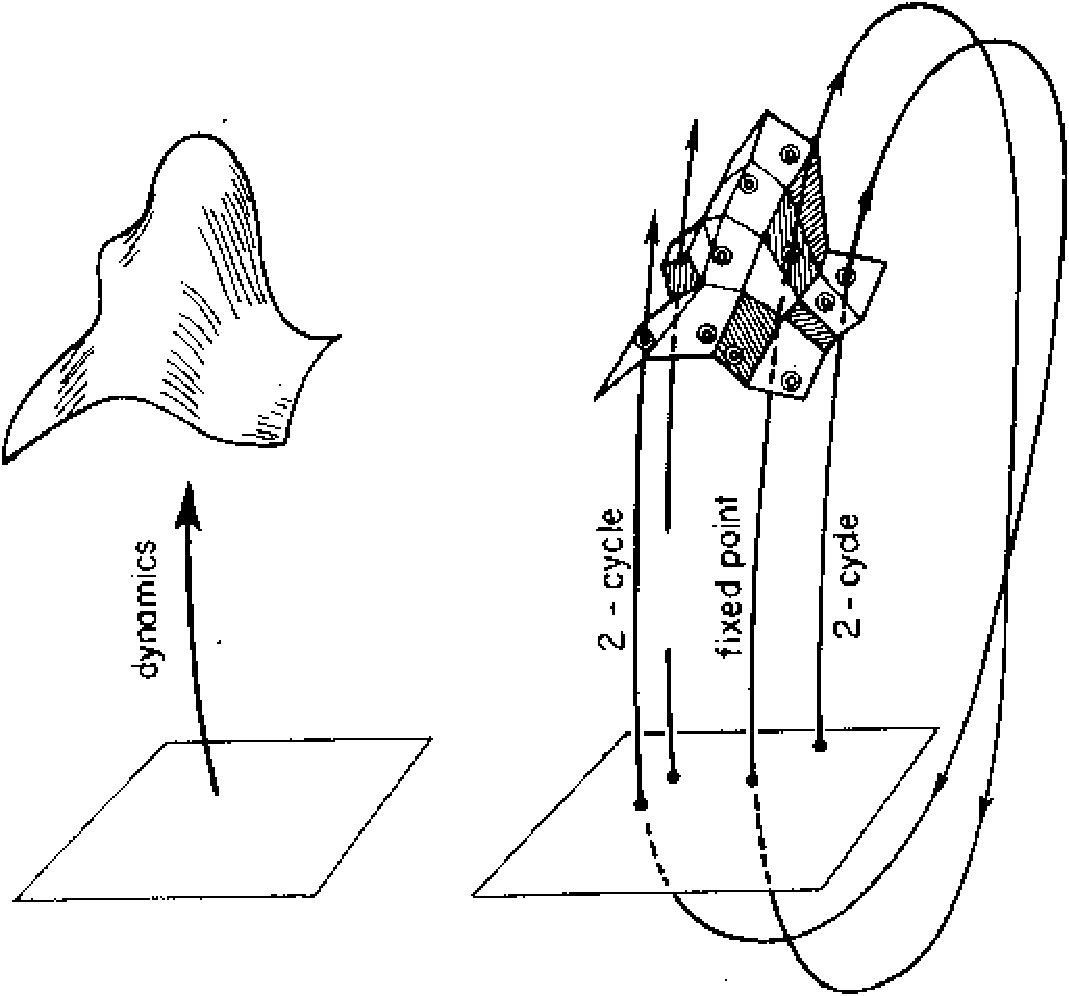
\includegraphics[width=0.60\textwidth]{f_1_08_1}
\end{center}
this is the
periodic-orbit implementation of the idea of {\statesp\ tessellation}
\end{frame}

\section[Summary]{conclusions}

 \begin{frame}{summary}

\begin{block}{conclusion}
  \begin{itemize}
   \item 'gauge fixing' - no insight into geometry of flows
   \item symmetry reduction by \mslices:
   \\
   efficient, allows
   exploration of high-dimensional flows\\
hitherto unthinkable
  \end{itemize}
\end{block}

\begin{block}{to be done}
\begin{itemize}
  \item construct Poincar\'e sections
  \item use the information quantitatively (periodic orbit theory)
\end{itemize}
\end{block}
\end{frame}

\begin{frame}{take-home message}
if you have a symmetry
\begin{center}
\textcolor{red}{\Large use it!}
\end{center}

\bigskip\bigskip
without symmetry reduction, no understanding of fluid
flows, nonlinear field theories possible
\end{frame}

\begin{frame}{amazing theory! amazing numerics! hope...}
\begin{center}
  
\includegraphics[width=0.60\textwidth,clip=true]
                    {ProblemsPill}
\end{center}
\end{frame}


\section[flotsam]{flotsam}

\begin{frame}{triumph : all pipe flow solution in one happy family}
\slicep\ is typical turbulent state (breaks all symmetries)
\\
plot $N2\_M1, \cdots$, \reqva, unstable manifolds
%($\Reynolds =2400$, stubby $L=2.5D$ pipe)
	\begin{columns}[t]
	\column{.50\textwidth}
\begin{block}
  \centering
%\includegraphics[width=1.00\textwidth]
{1611M1PROJFULL}
\\
    all in the same projection
\\
    inset: an expanded view % near the upper branch
\\
    blue loop: $T=4.93$ \\ \rpo
\end{block}
	\column{0.50\textwidth}
\begin{block}
  \centering
%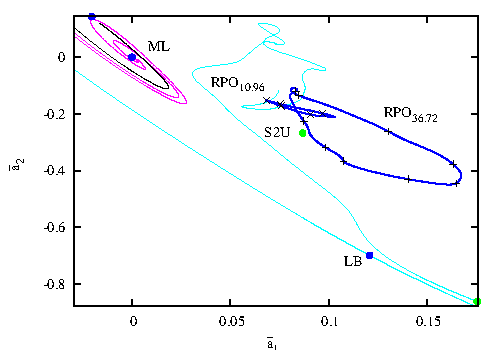
\includegraphics[width=1.00\textwidth]
{2803M1projOrb}
%\label{fig:M1Orb}
\\
      $T=10.96$ and $T=36.92$
\\
\rpo s
\\
embedded in turbulence
\end{block}
	\end{columns}
\bigskip
first 'turbulent' \rpo s for pipe flows!
\end{frame}

\begin{frame}{\rpo\ : \statesp\ visualization}
  \begin{columns}
  \column{0.55\textwidth}
%\includegraphics[width=1.0\textwidth,clip=true]
    {rpo}
  \column{0.45\textwidth}
		\only<1>{
\noindent
each cycle point
\begin{block}{}
\hfill
$\ssp_p (0) = \LieEl_p \ssp_p (\period{p} )
$ %\label{RPOrelper1}
\end{block}
exactly recurs at a fixed
\begin{block}{relative period} \hfill $\period{p}$
\end{block}
but shifted by a fixed
\begin{block}{group action} \hfill ${\LieEl_p}$
\end{block}
        }
		\only<2>{
\noindent
group action parameters
\\
$\gSpace = (\gSpace_1,\gSpace_2,\cdots\gSpace_N)$
are\\
irrational:

\bigskip

trajectory sweeps out ergodically the group orbit without
ever closing into a \po
        }
\end{columns}
		\only<1>{
{\scriptsize \textcolor{green}
{(green dashes) group orbit}\\
\textcolor{blue}{(blue) \rpo\ orbit}\\
(arrows) \textcolor{blue}{velocity}, \textcolor{green}{group} tangents
}
            }
\end{frame}

\begin{frame}{example: group orbit of a pipe flow  \reqv}
{\scriptsize
\slicep\ = Kerswell \emph{et al} $N2\_M1$ solution,
($\Reynolds =2400$, stubby $L=2.5D$ pipe)
}

\medskip

a very smooth, almost laminar solution

	\begin{columns}[t]
	\column{.45\textwidth}
			\begin{exampleblock}
{$\SOn{2}\times\SOn{2}$ symmetry
\\
$\Rightarrow$
group orbit is 2-torus}
projected on
  \begin{itemize}
    \item 2 \slicep\ group tangents
    \item 3. axis along the curvature direction
  \end{itemize}
			\end{exampleblock}
	\column{0.55\textwidth}
\begin{block}
  \centering
% \includegraphics[width=1.00\textwidth]{2839GOLB} %{2830GO7}
%  \caption{\label{fig:2830GO6}
    %\label{fig:M1groupOrb}
\end{block}
	\end{columns}

\bigskip
{\scriptsize
$2d$ group orbit (in 100,000 dimension \textcolor{red}{\statesp}) traced out by
  \begin{itemize}
    \item equal increment translations in $\theta$ (dashed blue)
    \item equal increments in $z$ (solid red)
  \end{itemize}
}
\end{frame}

\begin{frame}{example : pipe flow \rpo\ $\RPO{36.72}$}
symmetry reduction: full \statesp\ trajectory $\ssp(t)$

\begin{center}$\Rightarrow$\end{center}

\reducedsp\ trajectory $\sspRed(t)$, continuous
group induced drifts quotiented out
  \begin{columns}
  \column{0.5\textwidth}
\begin{block}{full \statesp}
 \begin{center}
%  \includegraphics[width=\textwidth]{2841GO3a}
 \end{center}
{\scriptsize traced for two periods:}
\\
{\scriptsize fills quasi-periodically
a highly contorted 2-torus }
\end{block}
  \column{0.5\textwidth}
\begin{block}{\reducedsp}
 \begin{center}
%  \includegraphics[width=\textwidth]{2841GO3b}
 \end{center}
{\scriptsize
closes a \po\ in one period}
\end{block}
\end{columns}
\end{frame}

\begin{frame}{slice \& dice}
\begin{block}{flow reduced to a slice}
\begin{center}
  \includegraphics[width=0.45\textwidth,clip=true]
  {ReducTraj3}
\end{center}
\end{block}
\slice\ \pSRed\
through the slice-fixing point $\slicep$,
normal to the group tangent $\sliceTan{}$ at $\slicep$,
intersects
group orbits (dotted lines).
The full
\statesp\ trajectory $\ssp(\tau)$ and the \reducedsp\
trajectory $\sspRed(\tau)$ are equivalent up to a group rotation
$\LieEl(\tau)$.
\end{frame}

\begin{frame}{}
we shall refer to these states as \emph{\template s}, each represented in
the \statesp\ $\pS$ of the system by a \emph{\template\ point} $\slicep$

\medskip

together with the velocity field at this point, a template defines a
linear \Poincare section, an affine hyperplane $\sspRed \in \PoincS$,
\beq
    \vel(\slicep) \cdot (\sspRed - \slicep)= 0
\,,
\ee{locTransvVar1}
locally normal to the $\vel(\slicep)$ at the \template\ point $\slicep$
\end{frame}

\begin{frame}{}
each \Poincare section $\PoincS{}^{(j)}$, provides a local chart at
$\slicep{}^{(j)}$ for a neighborhood of an important, qualitatively
distinct class of solutions (2-rolls states, 3-rolls states, \etc)

\medskip
together they `Voronoi' tessellate  the curved manifold in which the
reduced strange attractor is embedded by a finite set of hyperplane tiles
\end{frame}

\begin{frame}{}
a \Poincare section is a ($d\!-\!1$)\dmn\ hyperplane. If we pick another
{\template} point $\slicep{}^{(2)}$, it comes along with its own
\Poincare section
\medskip

any neighboring pair of $(d\!-\!1)$\dmn\ \Poincare
sections intersects in a `ridge' (`boundary,' `edge'), a $(d\!-\!2)$\dmn\
hyperplane, easy to compute
\end{frame}

\begin{frame}{}
a global atlas so constructed should be
sufficiently fine-grained: each `chart' or `tile,' bounded by ridges to
neighboring \Poincare sections, should be sufficiently small

\medskip

physical task is to, for a given dynamical flow, pick a set of
qualitatively distinct {\template s} whose \Poincare sections are locally
tangent to the strange attractor
\end{frame}

\begin{frame}{\statesp\ tessellation by \po s}
    \begin{minipage}[b]{0.40\textwidth}
\begin{block}{}
two 1-cycles

\medskip

a 2-cycle that alternates
between the neighborhoods of the two 1-cycles,
shadowing first one of the
two 1-cycles, and then the other
%}{fig:Tesselate} %{Hyp} %{fig6} and {tr:fig6} in ChaosBook
\end{block}
    \end{minipage}
~~~~~~
    \begin{minipage}[b]{0.51\textwidth}
\begin{center}
\includegraphics[width=1.00\textwidth]{f_1_08_1}
\end{center}
    \end{minipage}
smooth dynamics  (left frame) tesselated by the skeleton of periodic
points, together with their linearized neighborhoods, (right frame)
\end{frame}


\end{document}
